% Manuscript for Information Systems (Elsevier), class elsarticle.
% The ACM sigconf version of the same text is kept in alt/main_acmsigconf.tex.
% Review copy: change the class options to [preprint,review,12pt] for double line spacing.
\documentclass[preprint,12pt]{elsarticle}

\usepackage{booktabs}
\usepackage{amsmath}
\usepackage{amssymb}
\usepackage{graphicx}
\usepackage{xcolor}
\usepackage{url}

\journal{Information Systems}

% long \texttt names (settings, image tags) otherwise overflow the page
\sloppy

\begin{document}

\begin{frontmatter}

\title{Where Vector Search Benchmarks Go Wrong:\\
A Controlled Comparison of pgvector and Qdrant}

\author[hu]{Engin Demir}
\ead{engindemir@cs.hacettepe.edu.tr}

\author[hu]{Halil Burak Pala}
\ead{halilburakpala26@hacettepe.edu.tr}

\affiliation[hu]{organization={Hacettepe University, Department of Computer Engineering},
            city={Ankara},
            country={Turkey}}

\begin{abstract}
Teams that build retrieval-augmented applications choose between adding vector search to a relational
database they already run, such as PostgreSQL with pgvector, and deploying a dedicated vector database
such as Qdrant. Benchmarks of this choice are easy to get wrong, and we use the two systems, both with
HNSW, to show how. On dedicated bare-metal nodes with 100K to 1M MS MARCO v2.1 passages in 1024 dimensions
and the 1{,}677 TREC Deep Learning 2021--2023 queries, we compare at matched recall and record engine time,
end-to-end time and server CPU time of every query. Latency and cost per query give different answers.
Qdrant's single-client latency is 3.1--3.4$\times$ lower than pgvector's with its default four segments, but
its CPU time per query is only about 1.4$\times$ lower, and about equal with eight segments, so most of the gap
is parallelism inside a query. A profile and counter decomposition at 1M vectors shows that pgvector reads
fewer vectors per query than Qdrant but spends about 2.3$\times$ the cycles per vector read, half of its cycles
outside distance computation and element loading. Storing pgvector vectors in half precision makes its index a
third of the size with no detectable loss of speed or recall; int8 quantization makes Qdrant 1.6$\times$ faster
per query. A connection pooler halves pgvector's p99 latency when clients outnumber cores but adds no throughput. With the
exact search of the same corpus as reference, approximate search at recall 0.95 keeps 98\,\% of the nDCG@10 on the judged
queries that the corpus can answer. We catalog ten measurement confounders and quantify each one; three of them overturned our own
earlier laptop conclusions. Every table is bound to a manifest, and one command regenerates the analyses from the raw results.
\end{abstract}

\begin{highlights}
\item Latency and CPU per query give different answers for pgvector and Qdrant
\item pgvector's CPU gap is a cost per vector read, not a number of distances
\item Half-precision storage cuts the pgvector index to a third at no loss of speed
\item A connection pooler halves pgvector's p99 under overload but adds no throughput
\item Every table is bound to a manifest and regenerated from the raw results
\end{highlights}

\begin{keyword}
vector databases \sep approximate nearest neighbor search \sep HNSW \sep pgvector \sep Qdrant \sep benchmarking methodology \sep concurrency \sep retrieval-augmented generation
\end{keyword}

\end{frontmatter}

%% =============================================================
\section{Introduction}
%% =============================================================

Retrieval-Augmented Generation (RAG) systems combine a large language model with an
external vector store that supplies relevant passages at query time~\cite{pan2024survey}.
Retrieval recall affects the quality of the generated answers, and query latency and
throughput affect how responsive the application is. Selecting a vector store has
therefore become a common engineering decision.

In practice there are two options. One is to extend a relational database with vector
search. pgvector~\cite{pgvector} is the most widely used extension of this kind. It
adds Hierarchical Navigable Small World (HNSW)~\cite{malkov2018} and IVFFlat indexes to
PostgreSQL, so vectors, metadata and transactions stay in one system. The other option
is a dedicated vector database management system (VDBMS). Qdrant~\cite{qdrant} is a
typical example. It is written in Rust, has its own segment-based storage engine, and
offers HTTP and gRPC interfaces.

Since both systems rely on HNSW, the differences between them lie in engineering
rather than in the search algorithm. For the same reason, the outcome of a comparison
depends heavily on how it is measured. The client library, the wire protocol, the
moment at which an index is considered built, the query set and the server
configuration all stand between the engine and the number that ends up in a table. Our
own first measurements were taken on a laptop, with a thread-based Python client and
default settings. They showed pgvector 1.6 to 3.7 times faster than Qdrant at 100K vectors
at equal $ef$ and Qdrant's throughput not growing with the number of clients. Neither result held up
when we repeated the measurements under controlled conditions
(Section~\ref{sec:confounders}).

Published work does not answer the question directly. Zhang et al.~\cite{zhang2024}
study pgvector's execution path in detail but compare it with Faiss and Milvus, not with
Qdrant. Pan et al.~\cite{pan2024survey} survey more than twenty VDBMSs without running
them against each other. ANN-Benchmarks~\cite{aumuller2020} is the standard way to
evaluate ANN algorithms, but it runs them in-process, so the database layer, the client
and the network protocol are outside its scope.

This paper makes the following contributions.
\begin{itemize}
  \item A controlled comparison of pgvector and Qdrant on dedicated bare-metal nodes
    with 100K, 500K and 1M 1024-dimensional vectors and real queries. Results are
    reported at matched recall, with engine-side and end-to-end latency for every
    configuration.
  \item A list of measurement confounders for vector database benchmarks, with the
    size of each one's effect: the query set, asynchronous index construction,
    indexing thresholds, build memory and parallelism, buffer pool size, the client
    stack and protocol, and client-side saturation (Section~\ref{sec:confounders}).
  \item A separation of latency from CPU cost per query at matched recall, using
    controlled Qdrant segment counts and search-thread limits, and a profile and counter
    decomposition of where a query's CPU goes in each engine, which shows that the gap in
    CPU is a cost per vector read and not a number of distances
    (Sections~\ref{sec:cpu} and~\ref{sec:causal}).
  \item A load study that adds to closed-loop throughput a Poisson open-loop experiment at
    fixed fractions of each system's capacity and a test of a connection pooler, which shows
    what limits each system's throughput and tail latency
    (Sections~\ref{sec:concurrency}, \ref{sec:openloop} and~\ref{sec:pooling}).
  \item A memory and storage study: the effect of PostgreSQL's buffer pool apart from the operating
    system's page cache, both systems under cgroup memory limits with a cold cache, and the
    effect of reduced-precision storage (\texttt{halfvec} and \texttt{int8}) on size, speed and recall
    (Sections~\ref{sec:memory} and~\ref{sec:quant}).
  \item A sensitivity analysis of ranking quality: how much nDCG@10 approximate search loses against
    exact search on the judged TREC queries that a 1M-passage corpus can answer, with a rule fixed before
    looking and an account of why absolute nDCG cannot be reported (Section~\ref{sec:ranking}).
  \item Measurements of sensitivity to HNSW construction parameters and to embedding
    dimensionality (prefix truncation of a single model).
  \item Provenance that can be checked: every experiment has a manifest with its code commit, jobs and
    file checksums, the harness and the analysis tools are pinned by tags, and one command regenerates
    the analyses and the generated sections of this paper from the raw results (Section~\ref{sec:provenance}).
\end{itemize}

%% =============================================================
\section{Background and Related Work}
%% =============================================================

\subsection{HNSW}

HNSW~\cite{malkov2018} is a multi-layer proximity graph. The upper layers are sparse
and allow long jumps across the data, and the lower layers are dense and used for local
refinement. Two parameters control construction: $M$, the number of neighbors kept per
node, and $ef_{construction}$, the size of the candidate list used during insertion.
At query time, $ef$ sets the size of the dynamic candidate list. A larger $ef$ explores
more of the graph and gives higher recall at higher latency. The two systems reach
different recall at the same $ef$, so we compare them along their recall--latency curves
instead of at equal $ef$.

\subsection{Architectural Differences}

\textbf{Storage.} pgvector stores each vector as a column value in an ordinary
PostgreSQL heap tuple and keeps its HNSW graph in index pages managed by the shared
buffer pool~\cite{pgvector,postgres_docs}. A 1024-dimensional \texttt{vector} value is
about 4\,KB, which is larger than PostgreSQL allows inside a heap tuple, so the value is
moved out of line into the table's TOAST relation. We checked this for every table; from
100K to 1M the heap is 1.1\% of the size of the TOAST relation. Our query returns only
\texttt{id}, so an index scan reads the heap tuple but never fetches the vector from
TOAST. Qdrant divides a collection into segments. Each segment has its own vector
storage and HNSW graph, kept in memory or memory-mapped from disk~\cite{qdrant}.

\textbf{Index construction.} pgvector builds the HNSW graph with a separate
\texttt{CREATE INDEX} statement after the rows are loaded. The build can use parallel
maintenance workers and runs in memory as long as the graph fits in
\texttt{maintenance\_work\_mem}. Qdrant writes incoming points to appendable segments,
and a background optimizer builds their HNSW indexes later. It does so only for
segments larger than an indexing threshold (20\,MB by default), and smaller segments
are searched exhaustively~\cite{qdrant}. As a result, an upsert call returns before the
index is complete.

\textbf{Query path and concurrency.} PostgreSQL handles each connection in its own
backend process, and queries arrive over PostgreSQL's binary wire protocol. Qdrant runs
as a single multi-threaded process, accepts HTTP/JSON and gRPC requests, and searches the
segments of a collection in parallel.

\subsection{Prior Empirical Work}

Zhang et al.~\cite{zhang2024} ask whether relational systems have fundamental
limitations for vector search. Their case study compares PASE, a PostgreSQL-based
vector extension, with Faiss; pgvector is not the system they analyze. They identify
seven root causes of the gap, among them the cost of going through the buffer manager
and page-based indirection when all data is in memory (RC\#2), limited intra-query
parallelism (RC\#3), and a page-oriented layout that wastes space for HNSW
(RC\#4). They conclude that the gap is due to implementation issues and that there is no
fundamental limitation in relational databases. We test whether the first three causes
carry over to pgvector, a different and more widely used extension, and we compare it
with a specialized system under a database-level protocol. Pan et al.~\cite{pan2024survey} survey VDBMS
designs and treat the recall--latency tradeoff as the central issue. Aumüller et
al.~\cite{aumuller2020} define the usual methodology for comparing ANN algorithms, with
recall--throughput curves and exact ground truth. We follow the same methodology and
apply it at the database level. Suites that do benchmark full database systems exist,
for example VectorDBBench~\cite{vectordbbench}, an open-source tool maintained by the
vendor of Milvus that includes pgvector and Qdrant clients and reports throughput,
latency and cost-normalized scores. Such suites rank systems under their own default
configurations and client libraries. We instead ask which measurement choices change the
ranking, and we hold the protocol, recall level and hardware fixed while varying them.

\subsection{Systems and Indexes Outside This Study}
\label{sec:outside}

The comparison here is between two systems that both use an in-memory HNSW graph with
float32 vectors, so that the measurement choices can be isolated. Several lines of work
change the answer to the question that motivates it, and we do not measure them.

\textbf{Other vector database systems.} Milvus~\cite{milvus2021} is a purpose-built vector
data management system. VBase~\cite{vbase2023} targets queries that combine vector similarity
search with relational conditions, which is the integration that pgvector offers inside
PostgreSQL. VectorDBBench~\cite{vectordbbench}, discussed above, benchmarks several such
systems.

\textbf{Indexes for data larger than memory.} DiskANN~\cite{diskann2019} indexes, stores and
searches a billion-point collection on one machine with 64\,GB of RAM and a solid-state
drive. SPANN~\cite{spann2021} keeps the centroids of its posting lists in memory and the lists
on disk, and Starling~\cite{starling2024} is a disk-resident graph index framework for the
vector data held by one segment of a database. The Big-ANN competition at
NeurIPS~2021~\cite{bigann2022} ranked such algorithms at the scale of a billion vectors by
hardware cost, accuracy and throughput. Our largest collection holds one million vectors
and our out-of-core study (Section~\ref{sec:memory}) runs an in-memory graph from a
spinning disk, which is not the setting these indexes are designed for.

\textbf{Filtered search.} Filtered-DiskANN~\cite{filtereddiskann2023} and
ACORN~\cite{acorn2024} study nearest-neighbor search under attribute filters, with ACORN built
on HNSW. Filtered search is common in multi-tenant retrieval-augmented generation, and we do
not measure it (Section~\ref{sec:threats}).

\textbf{PostgreSQL-native alternatives.} pgvectorscale~\cite{pgvectorscale} extends pgvector
with a StreamingDiskANN index and with statistical binary quantization.
VectorChord~\cite{vectorchord} is a PostgreSQL extension whose index compresses vectors with
RaBitQ~\cite{rabitq2024}. Both target the cost of float32 HNSW indexes on large collections,
which is the cost this study measures (index size, build time, memory pressure), and their
authors report large improvements from vendor-run benchmarks that we have not reproduced.
pgvector's own half-precision and binary vector types, and Qdrant's scalar, product and
binary quantization, belong to the same group. A system comparison that excludes them
answers the question of which float32 HNSW implementation is cheaper, and not the question
of which system a team should deploy.

%% =============================================================
\section{Methodology}
%% =============================================================

\subsection{Problem and Metrics}

Given a corpus $\mathcal{D}=\{x_1,\dots,x_N\}\subset\mathbb{R}^d$ and a query $q$, the
$k$-nearest-neighbor problem under cosine similarity is
\begin{equation}
\text{KNN}(q,k)=\arg\max_{S\subseteq\mathcal{D},|S|=k}\sum_{x\in S}
\frac{q\cdot x}{\|q\|\,\|x\|}.
\end{equation}
Corpus vectors have unit norm up to $10^{-4}$ (the first 10{,}000 norms lie between 0.99994
and 1.00007), and vectors truncated to fewer dimensions are normalized again, so cosine
similarity is the inner product up to that precision. We compute exact ground truth over the
whole corpus in single precision with batched matrix products. Ties at rank $K$ are broken
arbitrarily and not by a fixed rule, and we did not count how many queries have such ties,
so a returned neighbor with the same score as a ground-truth neighbor may count as a miss.
Recall@$K$ is
\begin{equation}
\text{Recall@}K=\frac{|\mathcal{R}_K\cap\mathcal{G}_K|}{K},
\end{equation}
where $\mathcal{R}_K$ is the returned set and $\mathcal{G}_K$ the exact top-$K$. We use
$K=10$. Recall is the only quality measure of the main experiments; Section~\ref{sec:ranking} relates it to
nDCG@10 on the judged queries that the corpus can answer. We report mean and 99th-percentile (p99) latency, throughput, index build time,
index size, and the engine-side execution time per query for every measurement window.
Every query returns identifiers only. The pgvector query selects the \texttt{id} column. The
three Qdrant paths set the payload off explicitly and do not request vectors, which is the
default of the client library, and the raw gRPC request leaves that field unset. We checked
these defaults in the client but did not inspect what the server returns.

\subsection{Dataset and Queries}

The corpus consists of the first $10^6$ passages of MS MARCO v2.1~\cite{msmarco} with
1024-dimensional Cohere embed-english-v3.0 embeddings
(\texttt{CohereLabs/msmarco-v2.1-embed-english-v3})~\cite{cohere2024}. The 100K and 500K
corpora are prefixes of the 1M corpus. As queries we use the 1{,}677 TREC Deep Learning
2021--2023 queries that come with the same collection, embedded with the query input
type of the same model. None of the queries appears in the corpus. For the
dimensionality experiments we truncate corpus and query vectors to their first $d$
components and normalize them again. To our knowledge, Cohere embed-v3 was not trained with a
Matryoshka objective, so these truncated vectors need not behave like native low-dimensional
embeddings. Table~\ref{tab:dataset} summarizes the data.

\begin{table}[h]
  \caption{Dataset}
  \label{tab:dataset}
  \small
  \begin{tabular}{lr}
    \toprule
    Property & Value \\
    \midrule
    Corpus & MS MARCO v2.1 passages, first $10^6$ \\
    Embedding model & Cohere embed-english-v3.0 \\
    Dimensions & 1024 (truncated for E3) \\
    Queries & 1{,}677 (TREC DL 2021--2023) \\
    Words per passage (mean/median) & 161.7 / 155 \\
    \bottomrule
  \end{tabular}
\end{table}

\subsection{Experiment Map}

Table~\ref{tab:expmap} lists the experiments, which the results sections refer to by
label.

\begin{table}[t]
  \caption{Experiments}
  \label{tab:expmap}
  \small
  \begin{tabular}{p{0.07\columnwidth}p{0.85\columnwidth}}
    \toprule
    ID & Scope \\
    \midrule
    E1 & Scale (100K, 500K, 1M): recall--latency sweeps, three client protocols for Qdrant,
         closed-loop concurrency \\
    E2 & Eight HNSW construction settings $(M, ef_{construction})$ at 500K \\
    E3 & Embedding dimensionality (128--1024) and Qdrant's indexing threshold \\
    E4 & PostgreSQL buffer pool size (its memory-limit part is replaced by E10) \\
    E5 & Build time: three builds per engine and scale on one node, engines interleaved \\
    E6 & Qdrant segment count (1, 2, 4, 8) and search threads (one or automatic), with
         server CPU time per query, against a one-graph pgvector reference; three builds
         per cell \\
    E7 & Distance-kernel probe on a pinned core (scalar, AVX2 and AVX-512 time per 1024-dimensional distance) and a pilot of the hardware counters \\
    E8 & The E2 settings rebuilt three times each with a 21-point $ef$ grid, interpolated
         to matched recall \\
    E9 & Ingestion configurations: pgvector logged and unlogged, Qdrant with larger
         batches, parallel streams and deferred indexing; WAL and disk writes recorded \\
    E10 & Cold start and steady state under 16, 8 and 4\,GB memory limits, full query set in random
         order, three repetitions; pgvector with two buffer-pool settings, Qdrant memory-mapped \\
    E17 & Planner plans (no query run) for 100K--1M vectors, 128--1024 dimensions and 18 values of $ef$ \\
    E18 & Per-query recall and recall across eight dimensions, three builds each, 100K vectors \\
    E19 & Where a query's CPU goes at 1M $\times$ 1024: perf profiles and hardware counters of pgvector,
         Qdrant with four segments and Qdrant with one segment, three builds each \\
    E20 & Reduced precision at 1M $\times$ 1024: pgvector \texttt{halfvec} and Qdrant \texttt{int8}
         against their float32 arms, three builds each \\
    E21 & pgvector through PgBouncer (transaction pooling, pool equal to the server cores) against direct connections,
         1, 8, 32 and 48 clients, three builds \\
    E22 & Poisson arrivals at 50, 80, 95 and 110\,\% of each build's closed-loop capacity, 90\,s windows with a 30\,s ramp,
         both engines, three builds each \\
    E23 & Ranking quality of approximate search against exact search on the 63 judged queries that have a relevant
         document in the 1M corpus (sensitivity analysis), three builds per engine \\
    \bottomrule
  \end{tabular}
\end{table}

Table~\ref{tab:sources} states, for each table and figure, how many builds it rests on, where
they ran and which $ef$ point it uses. The two engines are not always built on the same node,
and the tables that compare them say so.

\begin{table*}[t]
  \caption{Where each table and figure comes from. Nodes are Slurm compute nodes. Job numbers,
  commits and file checksums are in the manifests under \texttt{data-manifests/}. The records of
  E1--E5 predate the provenance system and lack commit and seed fields.}
  \label{tab:sources}
  \small
  \begin{tabular}{p{0.15\textwidth}p{0.04\textwidth}p{0.15\textwidth}p{0.31\textwidth}p{0.26\textwidth}}
    \toprule
    Table or figure & Exp. & Builds & Jobs and nodes & $ef$ point \\
    \midrule
    Table~\ref{tab:matched}, Figure~\ref{fig:recall} & E1 & one per engine and scale &
      six jobs, the two engines on different nodes: 100K \texttt{hamsi54} (pgvector) and
      \texttt{hamsi32} (Qdrant), 500K \texttt{hamsi125} and \texttt{hamsi33}, 1M
      \texttt{hamsi112} and \texttt{hamsi14} &
      latency interpolated in recall to 0.90 and 0.95 \\
    Figure~\ref{fig:throughput} & E1 & same builds &
      same jobs &
      smallest swept $ef$ with Recall@10 $\ge 0.95$: pgvector 192, 384, 512 and Qdrant 96,
      384, 384 at 100K, 500K, 1M \\
    Table~\ref{tab:build}, Figure~\ref{fig:build} & E5 & three per engine and scale, engines
      interleaved & one job (6416987), one node (\texttt{hamsi120}) & not applicable \\
    Table~\ref{tab:hnsw} & E8 & three per setting & 24 jobs, both engines in each job, 7 nodes &
      each build interpolated to Recall@10 = 0.95 on a 21-point grid \\
    Table~\ref{tab:cpu} & E6 & three per cell & 48 Qdrant jobs on 10 nodes and 6 pgvector jobs on
      2 nodes, in separate arrays & smallest swept $ef$ reaching 0.95 on a 21-point grid;
      recall 0.951--0.957 and not identical for the two engines \\
    Table~\ref{tab:ingest} & E9 & three per arm and scale & 6 jobs, each builds all six arms on
      one node, 3 nodes in total & not applicable \\
    Table~\ref{tab:sb} & E4 & one build and one run per row & four jobs: \texttt{hamsi85}
      (128\,MB), \texttt{hamsi13} (1\,GB), \texttt{hamsi31} (4\,GB), \texttt{hamsi7} (32\,GB) &
      fixed $ef=64$ and $ef=512$ \\
    Table~\ref{tab:caps} & E10 & three per system and limit & one job per system, limit and
      repetition, 8 nodes & fixed $ef=128$ \\
    Figure~\ref{fig:dims} & E3 & one per dimension and arm & one job (6415795), one node
      (\texttt{hamsi107}) & fixed $ef=64$ \\
    Table~\ref{tab:perquery} & E18 & three per dimension & 24 jobs, 3 nodes & smallest swept $ef$
      whose mean recall reaches 0.95 (grid 16--384) \\
    Table~\ref{tab:causal} & E19 & three per arm & 6 jobs (all arms of one system per job), 6 nodes,
      the two systems on different nodes & smallest swept $ef$ with rep-0 recall $\ge 0.95$ on an 8-point grid
      (128--640); timing from reps 1 and 2 \\
    Table~\ref{tab:openloop} & E22 & three per engine & 6 jobs, 6 nodes, the two engines on different nodes & matched-recall $ef$ of each build;
      load as a fraction of the closed-loop throughput at 32 clients \\
    Table~\ref{tab:pooling} & E21 & three, one pgvector build per job & 3 jobs, 3 nodes; the three connection modes run
      one after the other on each build & $ef=448$ (smallest swept with recall $\ge 0.95$ on every build) and $ef=64$ \\
    Table~\ref{tab:ranking} & E23 & three per engine & 6 jobs, 6 nodes, the two systems on different nodes &
      all ten swept $ef$ values; the matched point is the smallest with recall $\ge 0.95$ over all queries \\
    Table~\ref{tab:quant} & E20 & three per arm & 6 jobs (both arms of one system per job), 6 nodes,
      the two systems on different nodes & smallest swept $ef$ reaching 0.95 on a 21-point grid
      (interpolated); throughput at the matched and the fixed $ef=64$ \\
    Section~\ref{sec:planner} & E17 & one per size and dimension & 20 jobs, 3 nodes (E1 default-planner
      run: as above) & 18 values from 16 to 1000, plans only \\
    \bottomrule
  \end{tabular}
\end{table*}

Table~\ref{tab:commits} gives the code commit, the Slurm jobs and the number of tasks and nodes behind each experiment, and the result of its strict audit.
The commit of the harness that produced the raw results is kept in each manifest; the tables and figures are regenerated from the raw results by the analysis
tools of the tag \texttt{analysis-v2} (the command \texttt{make verify-paper} does this and compares with the tracked files).

\begin{table}[t]
  \caption{The code commit, Slurm job (array) and number of tasks and distinct nodes behind each experiment of the main text, and the strict
  audit of its raw results (files / errors / warnings). The records of E1--E5 predate the provenance system and have none of these fields.
  Every manifest is in \texttt{data-manifests/}.}
  \label{tab:commits}
  \small
  \begin{tabular}{@{}llrrrr@{}}
    \toprule
    Exp. & commit & job(s) & tasks & nodes & audit \\
    \midrule
    E6 & \texttt{9050d65} & 6985667/6985669 & 54 & 11 & 54 / 0 / 0 \\
    E8 & \texttt{fe88da1} & 6996492 & 24 & 7 & 48 / 0 / 0 \\
    E9 & \texttt{31de7f4} & 6998157 & 6 & 3 & 36 / 0 / 0 \\
    E10 & \texttt{0b0b905} & 7008319 & 32 & 8 & 30 / 0 / 0 \\
    E17 & \texttt{a5bb141} & 7013754 & 20 & 3 & 20 / 0 / 0 \\
    E18 & \texttt{7d1b1c4} & 7014911 & 24 & 3 & 48 / 0 / 0 \\
    E19 & \texttt{518a444} & 7045635 & 6 & 6 & 9 / 0 / 0 \\
    E20 & \texttt{77f7567} & 7041536 & 6 & 6 & 12 / 0 / 0 \\
    E21 & \texttt{2516ade} & 7050273 & 3 & 3 & 3 / 0 / 0 \\
    E22 & \texttt{6e94ecd} & 7061154 & 6 & 4 & 6 / 0 / 0 \\
    E23 & \texttt{5276f14} & 7048647 & 6 & 2 & 6 / 0 / 0 \\
    \bottomrule
  \end{tabular}
\end{table}

\subsection{Environment}
\label{sec:env}

All experiments run on compute nodes of the TRUBA/ARF cluster, and each measurement has
a node to itself. A node has two Intel Xeon Gold 6258R processors (2$\times$28 cores,
2.7\,GHz, simultaneous multithreading disabled) and 187\,GB of memory, and runs Rocky
Linux 9.2 (kernel 5.14) with the \texttt{performance} frequency governor. Jobs are
scheduled by Slurm 23.02 with cgroup-v2 confinement. Database files are placed on the
node-local disk, a rotational drive behind a RAID controller. Measured with
\texttt{O\_DIRECT}, it writes 167\,MB/s sequentially and serves a random 8\,KiB read in
4.8\,ms (median), about 200 reads per second at queue depth one. The nodes we used have no NVMe device: \texttt{lsblk} on two \texttt{hamsi} nodes, one \texttt{barbun} node and the \texttt{smp} node shows a single rotational disk behind a RAID controller, and \texttt{/tmp} is on it (\texttt{docs/STORAGE\_CHECK.md}). The only other storage on a \texttt{hamsi} node is a 93\,GB \texttt{tmpfs} in memory. The cluster's documentation states that \texttt{/tmp} is NVMe on all servers; this holds on the one \texttt{orfoz} node we checked (a 894\,GB NVMe device) but not on the nodes above. Every result that depends on storage is therefore for a rotational disk, a worst case, and we did not repeat it on the \texttt{orfoz} partition, whose processors differ. Both engines run from Apptainer 1.3 images pinned by digest:
PostgreSQL 17.11 with pgvector 0.8.6 (\texttt{pgvector/pgvector:0.8.6-pg17}) and Qdrant
1.19.1 (\texttt{qdrant/qdrant:v1.19.1}).

The server is pinned to 8 cores of socket~0 and the client to the 28 cores of socket~1,
so the client never competes with the engine for cores or last-level cache. Each result
file records the node, the CPU topology, the kernel, the image digests and the complete
engine configuration.

\textbf{Configuration.} Unless stated otherwise, both systems build HNSW with $M=16$ and
$ef_{construction}=64$. These are pgvector's defaults; Qdrant's default
$ef_{construction}$ is 100, so we set it explicitly. PostgreSQL is configured for an
in-memory working set and parallel index builds: \texttt{shared\_buffers}=32\,GB,
\texttt{effective\_cache\_size}=64\,GB, \texttt{maintenance\_work\_mem}=16\,GB and
7 parallel maintenance workers. We also set the table's \texttt{parallel\_workers} to 7,
because PostgreSQL otherwise chooses the number of build workers from the heap size, and
the heap holds only the TOAST pointers. In addition, \texttt{jit} is off,
\texttt{track\_io\_timing} is on and \texttt{pg\_stat\_statements} is loaded. pgvector's
\texttt{hnsw.iterative\_scan} is off (its default), with \texttt{hnsw.max\_scan\_tuples} at
20{,}000 and \texttt{hnsw.scan\_mem\_multiplier} at 1; the benchmark query has no filter, so
iterative scans would not change its result. The CPU (Xeon Gold 6258R) supports AVX2 and AVX-512 (Section~\ref{sec:cpu}
reports instruction counts). We read the build records from the images (\texttt{docs/BUILD\_INFO.md}). The pgvector
library is compiled for baseline x86-64 with GCC 12.2 at \texttt{-O2} and has FMA clones of its distance functions that are
selected at run time, but no AVX-512 clone; the profiles of Section~\ref{sec:causal} show the FMA clone (\texttt{VectorInnerProduct.fma})
for 32-bit vectors. The Qdrant binary (rustc 1.98, clang 14) tests for AVX, FMA and AVX-512 at run time; the profile of the 32-bit path shows
its AVX kernel. Both engines therefore compute 32-bit distances with AVX/FMA code, and a difference between them is not one of AVX-512 against AVX2.
Qdrant runs with its defaults: vectors in memory, the default optimizer (indexing threshold 20\,MB)
and an automatically chosen number of segments.

\subsection{Measurement Protocol}
\label{sec:protocol}

\textbf{Build.} For pgvector we load the data with a single-stream binary \texttt{COPY}
into \texttt{items(id bigint primary key, embedding vector(d))} and then run
\texttt{CREATE INDEX}. For Qdrant we upload over gRPC in a single stream with batches of
512 points and then poll until the collection reports \texttt{green} on three
consecutive checks. Build time is load plus index time for pgvector and upload plus the
indexing wait for Qdrant. We also record how many vectors Qdrant actually indexed.

\textbf{Clients.} pgvector is queried through psycopg~3 with binary parameters and
prepared statements. Qdrant is queried in three ways. \emph{gRPC-lean} calls the
generated protobuf stub directly, \emph{gRPC} uses the official Python client, and
\emph{REST} uses the official client over HTTP/JSON. The per-call overhead of gRPC-lean
is close to that of psycopg, so it gives the fairest view of the engine. The other two
show what users of the official client experience.

\textbf{Latency sweep.} We sweep $ef\in\{16,32,64,96,128,192,256,384,512,768\}$ for
each client path. Each point uses one persistent connection, 500 untimed warm-up queries
drawn from the corpus, and then three sequential passes over all 1{,}677 queries. For
pgvector we record the custom and the generic query plan at every $ef$ and set
\texttt{enable\_seqscan=off}, as the pgvector documentation suggests, so that every
measurement uses the HNSW index. Section~\ref{sec:confounders} explains why this is
needed.

\textbf{Concurrency.} We run a closed loop with $C\in\{1,2,4,8,16,32,48\}$ client
\emph{processes}, each holding one persistent connection. Once all clients are
connected they send queries back to back. We discard the first 5\,s and measure the next
30\,s. Throughput counts the queries completed in the window, and latency statistics
cover the queries started in it. Each engine is run at a fixed $ef=64$ and at the
smallest swept $ef$ that reaches Recall@10 $\geq 0.95$ for that engine (matched recall).

\textbf{Engine-side time and telemetry.} For every window we record the engine-side
execution time per query (from \texttt{pg\_stat\_statements} for PostgreSQL and from
request telemetry for Qdrant), shared-buffer hits and reads per query, server and client
CPU time from \texttt{/proc}, voluntary and involuntary context switches, and user-level
hardware counters from \texttt{perf stat}. For PostgreSQL we also sample the wait events
of active backends every 10\,ms.

\textbf{Memory pressure.} This experiment has two parts, both at 1M vectors. In the
first, PostgreSQL runs with \texttt{shared\_buffers} of 128\,MB (the PostgreSQL
default), 1\,GB, 4\,GB and 32\,GB and no memory limit, so the whole index stays in the
operating system's page cache. Each setting gets the full latency sweep and concurrency
runs with $C\in\{1,8,32\}$. In the second part (E10), pgvector (with 1\,GB of shared buffers and, in a second
arm, with shared buffers set to a quarter of the limit) and Qdrant (with vectors and HNSW
graph memory-mapped from disk) are measured without a limit and under cgroup limits of 16,
8 and 4\,GB. For every system, limit and repetition we start a separate Slurm job. It builds
the index, stops the server, evicts its data files from the page cache with
\texttt{posix\_fadvise}, checks with \texttt{fincore} that nothing is left resident, and
restarts the server as a separate Slurm step with the memory limit. One client then runs
three passes over all 1{,}677 queries at $ef=128$, each pass visiting every query once in
a random order that depends on the repetition. The first pass has no warm-up and measures
the cold start; the later passes measure the steady state. For each pass we record
latency, recall, major and minor page faults, bytes read from storage and resident memory
of the server, and for each run the memory use of the server's cgroup. Each configuration
is run three times. A 2\,GB limit, which the earlier study included, is not repeated,
because with a spinning disk both systems did not leave the cold start in it.

\subsection{Provenance and Reproducibility}
\label{sec:provenance}

The results come from many commits of the harness, one per experiment, because each experiment was gated by a smoke test, a pilot and a full run of the exact
commit that ran it. Re-running everything with one commit would take days of queue time and would not change a number, so we make a narrower promise in two parts.
Every raw result keeps the commit that produced it (\texttt{code\_commit}, with the worktree clean) in its file and in the manifest of its experiment, together with the Slurm jobs, the node,
the image digests and the checksums of the files (Table~\ref{tab:commits}). And every analysis, table and generated section of this paper is regenerated from the raw results by one set of
analysis tools, the one at the tag \texttt{analysis-v2}; the harness itself is pinned by the tag \texttt{harness-v1}, the last commit that changed what it does. The command \texttt{make verify-paper} regenerates the 18 tracked
analysis files and compares them with the tracked ones, checks that the generated sections of this paper are in it verbatim, checks the structure of the text, checks that every table and figure is bound to an experiment,
a manifest and an analysis file, recomputes the headline numbers of the abstract, discussion and conclusion and the cells of the hand-typed result tables from the analysis files, and runs the unit tests. At the tag it passes all 30 steps.

The command has limits that the paper states. It does not check the numbers that were typed into the prose of sections without a generator, apart from the headline numbers; those were copied from the analysis summaries by hand. The first run of the table check found four values that had been copied from a rounded display or computed from rounded cells, and they were corrected. The first experiments, E1 to E5, predate the provenance system and are bound to the archived results only through their checksums and the figure reproduction. One analysis, of the first open-loop
run, is regenerated with the tools of the commit that produced it, because the later tools implement a second protocol. The raw results themselves (about 3\,GB) are not in the repository; their checksums are in the manifests.

%% =============================================================
\section{Measurement Confounders}
\label{sec:confounders}
%% =============================================================

Our first measurements of the same two systems were taken on a laptop with Docker, a
thread-based Python client and default settings. They led to three conclusions. At equal
$ef$, pgvector's mean latency at 100K vectors was 1.6 to 3.7 times lower than Qdrant's
(2.2 times at $ef=64$), Qdrant built its indexes 3.5--4.7$\times$ faster, and Qdrant's
throughput did not increase with more clients while its p99 latency reached 864\,ms. None
of these conclusions holds under the protocol of Section~\ref{sec:protocol}
(Table~\ref{tab:laptop}). Table~\ref{tab:confounders} lists ten confounders with their
mechanism and measured effect. Nine are causes of the laptop results or problems found
while building the new harness, and the tenth, intra-query parallelism, only became
visible once the new harness could separate latency from CPU cost
(Section~\ref{sec:cpu}). Each of them is easy to introduce by accident, and each one
changes a result. Table~\ref{tab:checklist} turns the list into a checklist that states
how to detect each confounder and how this study avoids it.

\begin{table*}[t]
  \caption{The laptop measurements against the controlled harness, 100K vectors unless noted.
  Laptop values are from the archived course-project result files. Controlled values are from
  the first scale runs (E1) and the same-node build repetitions (E5), with real queries and
  persistent clients. Ratios compare the systems within each column. The latency rows compare
  at equal $ef$, which gives the two engines different recall (Section~\ref{sec:cpu} and
  Table~\ref{tab:confounders}), so they show the direction of the change and not a matched
  comparison.}
  \label{tab:laptop}
  \small
  \begin{tabular}{p{0.2\textwidth}p{0.36\textwidth}p{0.38\textwidth}}
    \toprule
    Measurement & Laptop harness & Controlled harness \\
    \midrule
    Mean latency, $ef=64$ &
      pgvector 2.99\,ms, Qdrant 6.55\,ms: pgvector 2.2$\times$ faster &
      pgvector 1.17\,ms; Qdrant 0.79\,ms with lean gRPC (1.5$\times$ faster than pgvector),
      1.62\,ms with the official gRPC client and 2.66\,ms with REST (pgvector 1.4$\times$ and
      2.3$\times$ faster) \\
    Same, other $ef$ &
      pgvector 3.7$\times$ faster at $ef=16$, 2.6$\times$ at 32, 1.6$\times$ at 128 &
      Qdrant (lean gRPC) 1.0$\times$, 1.2$\times$ and 1.8$\times$ faster at $ef=16$, 32 and 128 \\
    Recall@10, $ef=64$ &
      0.993 (pgvector), 0.998 (Qdrant), queries drawn from the corpus &
      0.889 (pgvector), 0.927 (Qdrant), TREC queries not in the corpus \\
    Build time, 100K / 500K / 1M &
      pgvector 545 / 2{,}131 / 5{,}412\,s, Qdrant 116 / 609 / 1{,}367\,s: Qdrant 4.7 / 3.5 /
      4.0$\times$ faster &
      pgvector 20 / 94 / 307\,s, Qdrant 18 / 178 / 370\,s: Qdrant 1.2$\times$ faster at 100K,
      pgvector 1.9 and 1.2$\times$ faster at 500K and 1M \\
    Throughput, 100K &
      1 / 10 / 50 clients: pgvector 33 / 177 / 184\,qps, Qdrant 29 / 35 / 28\,qps &
      1 / 8 / 48 clients: pgvector 861 / 6{,}406 / 6{,}217\,qps, Qdrant (lean gRPC) 1{,}233 /
      5{,}108 / 6{,}623\,qps \\
    p99 latency, Qdrant, highest client count &
      864\,ms with 50 clients (mean 116\,ms) &
      15\,ms with 48 clients (mean 7.2\,ms) \\
    \bottomrule
  \end{tabular}
\end{table*}

\begin{table*}[t]
  \caption{Confounders in vector database benchmarks and their measured effect}
  \label{tab:confounders}
  \small
  \begin{tabular}{p{0.2\textwidth}p{0.36\textwidth}p{0.38\textwidth}}
    \toprule
    Confounder & Mechanism & Measured effect (this study) \\
    \midrule
    Queries drawn from the corpus &
      Each query is its own nearest neighbor, a known-item search &
      Recall@10 at $ef=64$, 100K: above 0.99 with corpus queries vs.\ 0.889
      (pgvector) and 0.927 (Qdrant) with real queries \\
    Build time taken at upsert return; default \texttt{maintenance\_work\_mem} &
      Qdrant builds HNSW asynchronously after the upsert returns; pgvector's graph does
      not fit in 64\,MB of build memory &
      Old harness: Qdrant 3.5--4.7$\times$ faster to build at all scales. Fair harness
      (with the next row fixed), same node: pgvector 1.9$\times$ and 1.2$\times$ faster at
      500K and 1M, 1.17$\times$ slower at 100K (Table~\ref{tab:build}) \\
    Indexing threshold &
      Qdrant leaves segments below 20\,MB unindexed and scans them exhaustively, while
      reporting the collection as \texttt{green} &
      100K vectors: 0--5.8\% left unindexed depending on $d$, raising engine time by up to
      1.9$\times$ at $ef=64$ (3.3$\times$ at $ef=16$) and recall by up to
      2.3 points. This produces a non-monotonic latency curve over $d$ and explains the
      earlier 384-dimension ``anomaly'' (Section~\ref{sec:dims}) \\
    Planner fallback for TOASTed vectors &
      pgvector's HNSW cost estimate lowers its startup cost for out-of-line vectors only when
      the estimated pages visited at startup (index pages times the scan fraction) exceed the
      table's pages and the fraction is below 0.5; below that point the index is costed
      with random page reads, against a sequential scan of a heap that holds about 1.1\%
      of the data &
      500K, $ef=256$: parallel exact scan, recall 1.000 at 890\,ms per query
      against 3--5\,ms at the neighboring $ef$ values. Predicted index costs 10.5k
      ($ef=192$) and 13.3k ($ef=256$); recorded 10{,}516 and 13{,}324. At $ef=384$ the
      correction applies and the cost drops to 3{,}787. Exposure over the grid we ran:
      Section~\ref{sec:planner} \\
    Build workers sized from the heap &
      PostgreSQL plans parallel \texttt{CREATE INDEX} workers from the heap size, which
      excludes the TOASTed vectors &
      100K: 53.4\,s index build with planner-chosen workers, 13.9\,s with the table's
      \texttt{parallel\_workers} set to 7 \\
    Buffer pool size &
      With PostgreSQL's default \texttt{shared\_buffers} (128\,MB), most index pages are
      copied from the operating system's page cache on every query &
      1M, $ef=64$, whole index in the page cache: engine time 3.82\,ms vs.\ 1.41\,ms with
      32\,GB of shared buffers; 1{,}648 vs.\ 4{,}954\,qps at $C=8$
      (Section~\ref{sec:memory}) \\
    Client stack and protocol &
      Serialization and client-library work is timed as query latency &
      Same engine time (0.45\,ms, 100K, $ef=64$): 0.79\,ms gRPC-lean, 1.61\,ms official
      gRPC client, 2.66\,ms REST \\
    Thread-based client, connection per query &
      GIL contention and connection setup inside the timed region &
      Old harness: flat Qdrant throughput of 28--35\,qps. New harness: linear scaling to
      8 clients, plateau when the 8 server cores are saturated \\
    Comparing at equal $ef$ &
      The engines reach different recall at the same $ef$ &
      $ef=64$ at 100K: pgvector 0.889 vs.\ Qdrant 0.927; fixed-$ef$ throughput favors the
      lower-recall engine \\
    Intra-query parallelism and segment count &
      Qdrant searches the segments of a collection in parallel, so more segments lower
      single-client latency while raising the work done per query &
      Matched recall 0.95, 1M: latency ratio 4.4$\times$ but CPU-per-query ratio
      1.0$\times$ with eight segments, against 2.9$\times$ and 1.7$\times$ with one
      (Section~\ref{sec:cpu}) \\
    \bottomrule
  \end{tabular}
\end{table*}

\begin{table*}[t]
  \caption{Checklist for benchmarking vector databases: how to detect each confounder and
  how this study avoids it}
  \label{tab:checklist}
  \small
  \begin{tabular}{p{0.2\textwidth}p{0.37\textwidth}p{0.37\textwidth}}
    \toprule
    Confounder & How to detect it & How this study avoids it \\
    \midrule
    Queries drawn from the corpus &
      Check whether query vectors appear in the corpus; recall near 1 at small $ef$ &
      Real TREC DL queries, none of which is in the corpus \\
    Build time at upsert return &
      Compare the point count with the indexed-vector count after the upload &
      Wait until the optimizer is idle and all vectors are indexed; a run fails
      otherwise \\
    Indexing threshold &
      \texttt{green} does not imply indexed: compare the indexed-vector count with the
      point count &
      Record both counts for every build; lower the threshold where the curve over $d$
      is studied \\
    Planner fallback &
      Record the query plan for every $ef$ and flag sequential scans &
      Plans are recorded per $ef$. The benchmark sets \texttt{enable\_seqscan = off}, so
      it measures the index and does not measure the exposure to the fallback \\
    Build workers sized from the heap &
      Compare the number of workers launched with the intended number &
      Set the table's \texttt{parallel\_workers} explicitly and record it \\
    Buffer pool size &
      Per-query buffer hits and reads from \texttt{pg\_stat\_statements}, separately from
      page-cache hits &
      Main results use a buffer pool that holds the index; the effect of the default is
      measured on its own \\
    Client stack and protocol &
      Record engine-side time and end-to-end time for the same queries &
      Report every protocol separately, with persistent connections and processes
      pinned to cores disjoint from the server \\
    Thread-based client &
      Client CPU use close to its allotment, flat throughput as clients are added &
      Multi-process clients; client cores busy are reported next to server cores \\
    Comparing at equal $ef$ &
      Compare recall at the settings being compared &
      Interpolate to matched recall, with a finer $ef$ grid near the target \\
    Intra-query parallelism &
      Server CPU time per query next to latency; segment count from the engine &
      Report CPU per query with latency, and control the segment count and search
      threads \\
    \bottomrule
  \end{tabular}
\end{table*}

%% =============================================================
\section{Results}
%% =============================================================

\subsection{Build Time}
\label{sec:build}

Build times turned out to depend on the node as much as on the system. In the scale
runs each engine was built on whichever node the scheduler assigned, and the same
build took noticeably different times on different nodes: pgvector at 500K took 144\,s
on one node and 88--98\,s on another, and Qdrant at 1M took 283\,s on one node and
362--383\,s on another. Both systems write their data and write-ahead logs to the
node-local disk, which is a spinning drive, so some of this variation likely comes from
the disks. We therefore repeated every build three times on a single node, alternating
the two engines, and report only these runs (Table~\ref{tab:build},
Figure~\ref{fig:build}).

On the same node, pgvector's load and \texttt{CREATE INDEX} take 20.4, 93.7 and 307\,s
at 100K, 500K and 1M, and Qdrant's upload and indexing take 17.5, 178 and 370\,s. Qdrant
is 1.17$\times$ faster at 100K, and pgvector is 1.9$\times$ faster at 500K and
1.2$\times$ faster at 1M. The standard deviation of the total build time across the three
builds is at most 13\% of the mean. Qdrant indexes segments while the upload is still running, and only
4--10\% of its build time falls after the last upsert returns, so its total is almost
entirely the single-stream gRPC upload. pgvector's index build is its larger phase at
every scale. Its load time grows faster than the data at 1M (98.5\,s against 26.4\,s at
500K). Section~\ref{sec:ingest} below shows why, and shows that this comparison depends on how
each system is loaded.

\begin{table*}[t]
  \caption{Build time (s, mean $\pm$ standard deviation of three builds on one node,
  engines interleaved) and pgvector index size (GiB).}
  \label{tab:build}
  \small
  \begin{tabular}{r|rrrr|rrr}
    \toprule
     & \multicolumn{4}{c|}{pgvector} & \multicolumn{3}{c}{Qdrant} \\
    $N$ & load & index & total & GiB & upload & wait & total \\
    \midrule
    100K & 4.9 $\pm$ 0.9 & 15.6 $\pm$ 1.7 & 20.4 $\pm$ 2.6 & 0.76 & 15.8 $\pm$ 0.4 & 1.7 $\pm$ 0.6 & 17.5 $\pm$ 0.9 \\
    500K & 26.4 $\pm$ 2.9 & 67.3 $\pm$ 4.1 & 93.7 $\pm$ 4.9 & 3.81 & 168.2 $\pm$ 1.3 & 9.8 $\pm$ 1.3 & 178.0 $\pm$ 2.7 \\
    1M & 98.5 $\pm$ 0.9 & 208.8 $\pm$ 10.8 & 307.3 $\pm$ 11.7 & 7.61 & 356.2 $\pm$ 14.3 & 14.1 $\pm$ 4.9 & 370.2 $\pm$ 11.1 \\
    \bottomrule
  \end{tabular}
\end{table*}

\begin{figure}[h]
  \centering
  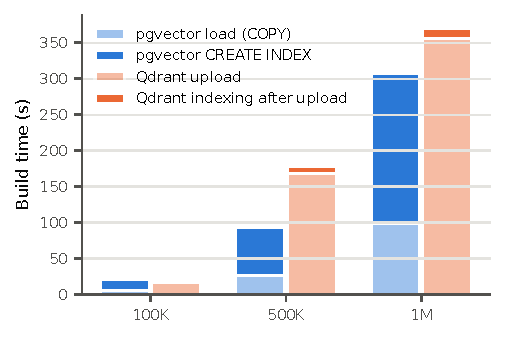
\includegraphics[width=\columnwidth]{figures/build_time.pdf}
  \caption{Build time by phase, mean of three builds on one node. Light segments: data
  ingestion (pgvector \texttt{COPY}, Qdrant upload); dark segments: index construction
  after ingestion.}
  \label{fig:build}
\end{figure}

The size of pgvector's index does not change with $M$. At 500K it is 3.81\,GiB for
$M=16$, 32 and 64. The byte budget explains this. An 8\,KiB page offers 8{,}156\,bytes for one
tuple, and 8{,}160 for tuples in general once the 24-byte page header and 8-byte page special
space are taken out. An element tuple is a 72-byte header (type and flags, ten heap
pointers of 6 bytes, the neighbor pointer) followed by the vector, which is 8 bytes of
header plus 4 bytes per dimension. At 1024 dimensions it takes 4{,}176 bytes after
alignment, so a second element (8{,}360 bytes with item identifiers) does not fit on the
page, and the index uses one page per vector. A level-0 neighbor tuple holds $2M$ pointers
of 6 bytes and a 4-byte header, which is 200, 392 and 776 bytes for $M=16$, 32 and 64.
Each fits in the 3{,}980 bytes that remain beside the element, so a larger $M$ costs no
extra page. The same budget gives two elements per page at 768 dimensions (3{,}152 bytes
each), and the measured index of 249{,}433 pages for 500K vectors (E17) is half a page per
vector, as predicted. Qdrant has no such constraint. We read the layout from the
\texttt{hnsw.h} header of pgvector 0.8.0 and checked that the tuple definitions are identical in
0.8.6, where only the size macros changed, to guard against overflow.

\subsection{Ingestion Fairness}
\label{sec:ingest}

The comparison above sets pgvector, with parallel index-build workers and a large
maintenance memory, against a Qdrant load that uses one gRPC stream and batches of 512
points. We therefore built each system in several configurations on the same node (E9,
Table~\ref{tab:ingest}): pgvector with a logged and an unlogged table, and Qdrant with the
baseline upload, with batches of 4096 points, with four parallel streams, and with four
streams, batches of 4096 and indexing deferred until the upload ends. Each configuration
was built three times, interleaved on one node, with the order rotated between repetitions.
The baseline arms reproduce the builds above within 4\% at 1M (pgvector 296\,s against
307\,s, Qdrant 356\,s against 370\,s).

\begin{table*}[t]
  \caption{Build time by ingestion configuration (s, mean $\pm$ standard deviation of three
  builds on one node). pgvector: load and \texttt{CREATE INDEX}. Qdrant: upload and wait for
  indexing. WAL and disk writes are totals in MB over load, index build and the final
  checkpoint.}
  \label{tab:ingest}
  \small
  \begin{tabular}{rl|rrr|rr}
    \toprule
    $N$ & Configuration & ingest & index & total & WAL MB & disk MB \\
    \midrule
    500K & pgvector, logged & 32.4 $\pm$ 2.8 & 74.4 $\pm$ 5.6 & 106.8 $\pm$ 7.5 & 4533 & 6909 \\
     & pgvector, unlogged & 11.2 $\pm$ 0.0 & 50.5 $\pm$ 0.2 & 61.7 $\pm$ 0.2 & 0 & 15 \\
     & Qdrant, baseline & 143.2 $\pm$ 18.0 & 8.7 $\pm$ 1.3 & 151.9 $\pm$ 19.1 & -- & -- \\
     & Qdrant, batch 4096 & 120.7 $\pm$ 7.5 & 12.1 $\pm$ 0.8 & 132.8 $\pm$ 8.3 & -- & -- \\
     & Qdrant, 4 streams & 97.8 $\pm$ 8.7 & 16.9 $\pm$ 5.9 & 114.7 $\pm$ 2.9 & -- & -- \\
     & Qdrant, tuned & 62.6 $\pm$ 1.4 & 36.4 $\pm$ 0.8 & 99.0 $\pm$ 1.5 & -- & -- \\
    \midrule
    1M & pgvector, logged & 93.0 $\pm$ 11.2 & 202.7 $\pm$ 17.6 & 295.8 $\pm$ 28.6 & 9067 & 13894 \\
     & pgvector, unlogged & 22.2 $\pm$ 0.1 & 103.6 $\pm$ 0.5 & 125.9 $\pm$ 0.6 & 0 & 46 \\
     & Qdrant, baseline & 339.0 $\pm$ 42.5 & 16.9 $\pm$ 5.1 & 355.9 $\pm$ 47.4 & -- & -- \\
     & Qdrant, batch 4096 & 271.1 $\pm$ 22.6 & 17.3 $\pm$ 4.6 & 288.4 $\pm$ 27.0 & -- & -- \\
     & Qdrant, 4 streams & 229.5 $\pm$ 30.4 & 20.0 $\pm$ 2.2 & 249.5 $\pm$ 32.5 & -- & -- \\
     & Qdrant, tuned & 130.3 $\pm$ 2.2 & 75.6 $\pm$ 2.6 & 205.9 $\pm$ 4.4 & -- & -- \\
    \bottomrule
  \end{tabular}
\end{table*}

\textbf{Qdrant's build time depends on how it is loaded.} Four parallel streams, batches of
4096 points and deferred indexing together cut the total from 152 to 99\,s at 500K
(1.5$\times$) and from 356 to 206\,s at 1M (1.7$\times$). Deferring indexing moves work from
the upload to the wait that follows (at 1M the wait grows from 17 to 76\,s), but the total
still falls.

\textbf{pgvector's load is limited by write-ahead logging.} At 1M the load writes 4.6\,GB of
WAL, about as much as the data itself, and the index build writes another 4.5\,GB. The
final checkpoint then writes 13.9\,GB in 80\,s, about 175\,MB/s, which matches the
167\,MB/s we measured for the node's disk. The load takes 2.9$\times$ longer at 1M than at
500K for twice the data, and a second checkpoint is requested during the 1M build (two,
against one in each of the other three pgvector configurations at 500K and 1M). With an unlogged table there is no
WAL, the load takes 11 and 22\,s and scales linearly (2.0$\times$), and the total falls to
62 and 126\,s, 1.7$\times$ and 2.3$\times$ faster than the logged table. The 1M load is
therefore limited by logging to the spinning disk. An unlogged table does not survive a
crash, so this arm shows how much of the cost is logging and is not a like-for-like
production configuration. We did not repeat the experiment on faster storage.

\textbf{Which system builds faster depends on the configurations compared.} Against
Qdrant's baseline upload, logged pgvector is 1.4$\times$ faster at 500K and 1.2$\times$
faster at 1M, as in the earlier table. Against Qdrant with parallel streams and deferred
indexing, the two are about equal at 500K (107 against 99\,s) and Qdrant is 1.4$\times$
faster at 1M (206 against 296\,s). An unlogged pgvector table is faster than every Qdrant
configuration (1.6$\times$ at both scales against the tuned arm). We therefore do not claim
that either system builds faster. The earlier statement that pgvector builds faster
describes Qdrant's single-stream baseline, and it reverses once Qdrant is loaded in
parallel.

\subsection{Latency at Matched Recall}

Figure~\ref{fig:recall} shows the recall--latency curves, end to end in the top row and
engine side in the bottom row. Table~\ref{tab:matched} reads the curves at two recall
targets. At every scale and target, Qdrant's single-client engine latency is
3.0--3.9$\times$ lower than pgvector's, with its default four segments searched in
parallel (Section~\ref{sec:cpu} separates this from CPU cost), and its p99 latency is
closer to its mean. End-to-end results depend on the
client path. With gRPC-lean, Qdrant remains 1.7--3.3$\times$ faster. With the official
gRPC client the advantage drops to 0.8--2.3$\times$, and with REST to 0.5--1.7$\times$.
At Recall@10 = 0.90, a Qdrant user on REST waits longer than a pgvector user at every
scale. Qdrant moves ahead over REST only at high recall and large scale, where pgvector's
engine time is the larger part of the total.

\begin{figure*}[t]
  \centering
  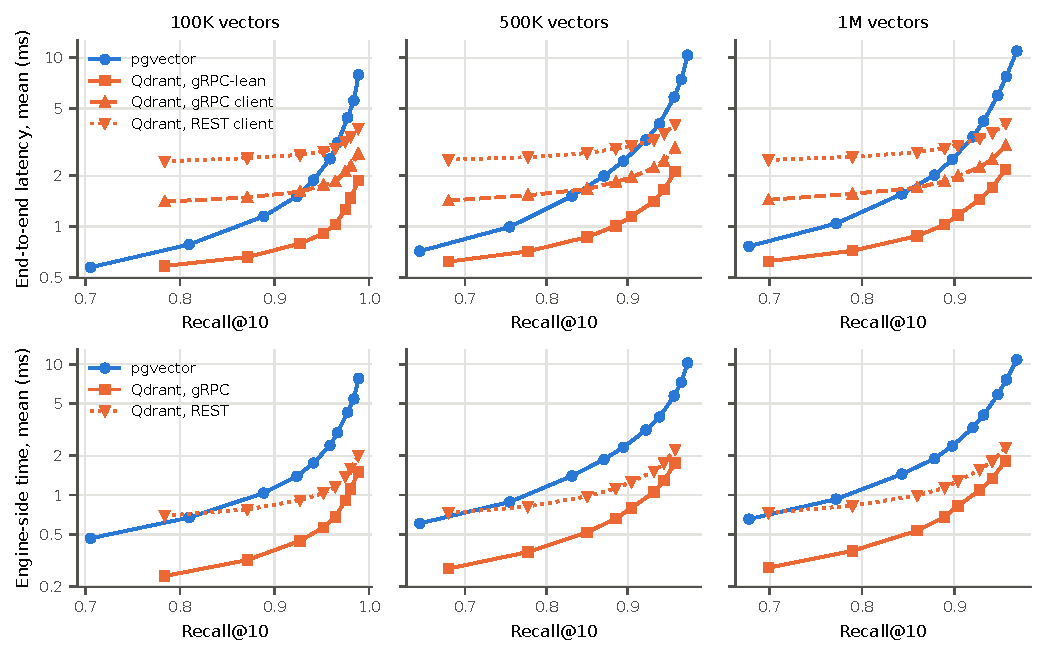
\includegraphics[width=\textwidth]{figures/recall_latency.pdf}
  \caption{Recall@10 against mean latency, end to end (top) and engine side (bottom),
  one point per $ef$ (mean of three passes over 1{,}677 queries). gRPC-lean and the
  official gRPC client share the same engine path.}
  \label{fig:recall}
\end{figure*}

\begin{table*}[t]
  \caption{Latency at matched Recall@10 (ms, log-linear interpolation between swept
  $ef$ values; three passes each, coefficient of variation of the mean at most 6\%).
  ``eng.'' is engine-side time.}
  \label{tab:matched}
  \small
  \begin{tabular}{rr|rrr|rrr|r|rr|r}
    \toprule
     & & \multicolumn{3}{c|}{pgvector} & \multicolumn{3}{c|}{Qdrant gRPC-lean} &
       gRPC client & \multicolumn{2}{c|}{REST client} & engine \\
    $N$ & Recall & mean & p99 & eng. & mean & p99 & eng. & mean & mean & eng. & speedup \\
    \midrule
    100K & 0.90 & 1.25 & 2.06 & 1.14 & 0.72 & 0.88 & 0.38 & 1.55 & 2.60 & 0.84 & 3.0$\times$ \\
    100K & 0.95 & 2.18 & 3.26 & 2.05 & 0.90 & 1.11 & 0.56 & 1.74 & 2.78 & 1.03 & 3.7$\times$ \\
    500K & 0.90 & 2.58 & 4.38 & 2.45 & 1.11 & 1.48 & 0.76 & 1.93 & 2.98 & 1.23 & 3.2$\times$ \\
    500K & 0.95 & 5.06 & 7.86 & 4.93 & 1.81 & 2.38 & 1.45 & 2.62 & 3.73 & 1.93 & 3.4$\times$ \\
    1M & 0.90 & 2.57 & 4.48 & 2.44 & 1.13 & 1.51 & 0.78 & 1.95 & 2.99 & 1.24 & 3.1$\times$ \\
    1M & 0.95 & 6.46 & 9.84 & 6.32 & 1.98 & 2.64 & 1.62 & 2.81 & 3.87 & 2.10 & 3.9$\times$ \\
    \bottomrule
  \end{tabular}
\end{table*}

Comparing the two rows of Figure~\ref{fig:recall} shows where the client cost arises.
The difference between end-to-end and engine time is about 0.1\,ms for psycopg and
0.35\,ms for gRPC-lean, and 1.1--1.2\,ms for the official gRPC client. Most of the time a
Python user of the official client waits is therefore spent in the client. REST also
adds work on the server. At the same $ef$, Qdrant's engine-side time over REST is
0.4--0.5\,ms higher than over gRPC, which we attribute to JSON parsing and
serialization.

\subsection{Planner Exposure}
\label{sec:planner}

The main experiments force the HNSW index (\texttt{enable\_seqscan = off}), so they measure
the index and not how often PostgreSQL's planner would choose it. We measured that exposure
separately (E17) without running any query. For one build of each combination of 100K, 250K,
500K, 750K and 1M vectors and 128, 384, 768 and 1024 dimensions, we ask the planner for the
plan of the benchmark query at 18 values of $ef$ from 16 to 1000, and we record its own
choice together with the cheapest index plan and the cheapest scan plan and their costs. Of
the 360 cells, 9 (2.5\%) use a sequential scan under the default planner.

All 9 are in the two dimensions whose vectors are stored out of line (768 and 1024), where
they make up 9 of 180 cells (5.0\%) and occur in 6 of the 10 builds. None occurs at 128 or
384 dimensions (0 of 180). Within the affected builds the exposure is a narrow range of
$ef$ and not a threshold: at 500K vectors and 1024 dimensions only $ef=256$ is affected, at
750K the values 384 and 448, and at 1M only 512, while the values on both sides of each use
the index. This agrees with the earlier run at the default planner, where only $ef=256$ at
500K was slow (Table~\ref{tab:confounders}), and it adds that the range moves with $N$
and the dimension, so a setting that is safe at one scale may not be at the next.

The cause is in pgvector's cost estimator (\texttt{hnswcostestimate} in \texttt{src/hnsw.c},
version 0.8.6). From $M$, $ef$ and the number of tuples it estimates the fraction of the index
that a scan visits, and it charges the pages visited at random-page cost. A comment in the
source notes that the TOAST pages are not part of the sequential scan cost, and for this reason
it lowers the startup cost only when the estimated pages visited at startup (the index pages
times that fraction) exceed the number of pages of the table, and only when the fraction is
below 0.5. When the vectors are stored out of line the table is small (3{,}712 pages at 500K
vectors, which hold pointers only), so the condition holds from a modest $ef$ on, and below it
the index is charged at the full random-page cost. In that band the index can cost more than a
parallel sequential scan of the small heap. We applied the formula from the source to the page
counts we recorded. It predicts, in all 20 builds, the value of $ef$ at which the cost of the
index plan drops: 320 at 500K vectors and 1024 dimensions, where the cost falls from 13{,}323
at $ef=256$ to 3{,}782 at $ef=320$, and no drop at all for the builds with 128 and 384
dimensions, whose heaps are large. The exposed values of $ef$ are the ones just below the
predicted threshold, where the uncorrected index cost exceeds the scan cost. The cost of the
scan plan depends on the heap, which has the same size at 768 and at 1024 dimensions, so the
scan costs exactly the same at both (for example 11{,}819 at 500K), and 3.0 to 3.8 times less
than at 128 dimensions with the same number of vectors, although it reads far more data. In the
affected cells the index plan costs 1.01 to 1.27 times as much as the scan plan.

Two limits apply. The plans are those of one prepared statement with a custom plan, and the
planner may choose differently for other query vectors or with a generic plan. And we
measured the latency of the scan plan only at 500K vectors and 1024 dimensions (888\,ms
against 4.1\,ms for the index, Table~\ref{tab:confounders}), not in the other eight cells.
We have not reported this behavior to the pgvector maintainers.

\subsection{Latency Versus CPU Cost}
\label{sec:cpu}

Single-client latency at matched recall does not separate how much work a query costs
from how many cores work on it. Qdrant searches the segments of a collection in
parallel, so a configuration with more segments finishes sooner while spending more
CPU time. We therefore ran Qdrant with 1, 2, 4 and 8 target segments and with the
search thread pool limited to one thread or left on its automatic setting, built each
configuration three times, and measured server CPU time per query next to latency at
Recall@10 of 0.95 (Table~\ref{tab:cpu}). The segment counts are optimizer targets. A
target of one yields a single non-empty indexed segment plus an empty appendable
segment, and all vectors were indexed in every run.

\begin{table}[t]
  \caption{Smallest swept $ef$ with Recall@10 $\ge 0.95$ (recall 0.951--0.957, not identical
  for the two engines), one client, lean gRPC. Latency and server CPU time per
  query in ms (mean of three builds); ratios are pgvector divided by Qdrant, so values
  above 1 favor Qdrant. 95\% intervals are in the analysis files.}
  \label{tab:cpu}
  \small
  \begin{tabular}{llrrrr}
    \toprule
    $N$ & Configuration & Latency & CPU & Lat.\ ratio & CPU ratio \\
    \midrule
    500K & pgvector              & 5.64 & 5.55 & --- & --- \\
         & Qdrant, 1 seg., auto  & 2.60 & 2.36 & 2.2 & 2.3 \\
         & Qdrant, 4 seg., auto  & 1.79 & 3.86 & 3.1 & 1.4 \\
         & Qdrant, 4 seg., 1 thr.& 3.93 & 3.68 & 1.4 & 1.5 \\
         & Qdrant, 8 seg., auto  & 1.49 & 6.00 & 3.8 & 0.9 \\
    \midrule
    1M   & pgvector              & 7.63 & 7.53 & --- & --- \\
         & Qdrant, 1 seg., auto  & 2.62 & 4.32 & 2.9 & 1.7 \\
         & Qdrant, 4 seg., auto  & 2.25 & 5.20 & 3.4 & 1.4 \\
         & Qdrant, 4 seg., 1 thr.& 5.12 & 4.87 & 1.5 & 1.5 \\
         & Qdrant, 8 seg., auto  & 1.72 & 7.43 & 4.4 & 1.0 \\
    \bottomrule
  \end{tabular}
\end{table}

Two findings stand out. First, the latency advantage grows with the number of segments
(up to 3.8$\times$ at 500K and 4.4$\times$ at 1M with eight segments), while the CPU
advantage shrinks and disappears at eight segments (0.9$\times$ and 1.0$\times$). The
latency ratio is therefore largely a measure of intra-query parallelism. Second, Qdrant
is still cheaper per query than pgvector with one segment (2.3$\times$ at 500K and
1.7$\times$ at 1M) and with the search pool limited to one thread (1.4--1.5$\times$ at
four segments), so the gap is not only parallelism. At the default of four segments the
work ratio is 1.4--1.5$\times$, much lower than the 3.1--3.4$\times$ latency ratio. The
intervals are wide for some Qdrant configurations because the matched-recall $ef$ varies
between builds, so we report these ratios as ranges and do not treat differences of
about ten percent as meaningful.

\subsection{Causal Decomposition}
\label{sec:causal}

Section~\ref{sec:cpu} shows that pgvector needs more CPU per query than Qdrant, and that Qdrant's
latency lead comes mostly from searching its segments in parallel. This section asks where a query's
CPU goes. One client queries 1M vectors of 1024 dimensions at the matched-recall $ef$ of each build (the
smallest swept $ef$ that reaches Recall@10 of 0.95). We built pgvector, Qdrant with its automatic segments
(four) and Qdrant with one segment, 3, 3 and 3 times. Timing uses repetitions one and two of the sweep; repetition
zero ran under \texttt{perf record} (user-space cycles of the server processes), and a separate
30\,s window gives user-space hardware counters per query. The profiles resolve function names only
after unpacking the images and pointing \texttt{perf report} at them, which we did for both. We sort the
functions into categories by name: the distance function, graph search with element loading, queues and
visited sets, the buffer manager (hash lookup, pinning, locks), and the rest. Inlining moves work between
categories, so a share is the share of samples whose top frame is in the category.

\begin{table*}[t]
  \caption{CPU per query at matched recall 0.95, one client, 1M vectors, mean of the builds.
  Cycles are user-space; the category columns are millions of cycles per query (profile share times
  cycles). Vector reads are cache misses per query divided by the 64 cache lines of a vector, a proxy
  checked against pgvector's block counter (5107 blocks per query). The last column sums the request path,
  the unresolved addresses and the rest.}
  \label{tab:causal}
  \small
  \begin{tabular}{@{}lrrrrrrrrrrr@{}}
    \toprule
    & & CPU & Mcyc. & & reads & cyc. per & \multicolumn{5}{c}{Mcycles per query in} \\
    arm & $ef$ & ms & per q. & IPC & $\times10^3$ & read & distance & elements & queues & buffers & other \\
    \midrule
    pgvector & 448 & 6.54 & 17.2 & 0.66 & 5.2 & 3342 & 4.5 & 4.3 & 1.0 & 4.4 & 3.0 \\
    Qdrant, 4 segments & 363 & 4.76 & 12.5 & 0.51 & 8.9 & 1410 & 9.6 & 1.7 & 0.3 & 0.0 & 0.9 \\
    Qdrant, 1 segment & 427 & 3.75 & 9.9 & 0.51 & 6.9 & 1427 & 7.5 & 1.4 & 0.3 & 0.0 & 0.7 \\
    \bottomrule
  \end{tabular}
\end{table*}

\paragraph{The gap is per-read cost, not the number of distances.}
pgvector uses 1.37 (1.31 to 1.52) times the CPU time per query of Qdrant with its automatic segments and 1.75 (1.68 to 1.88) times that of Qdrant with one
segment (ratio of means, with the range over all build pairs). It does not read more vectors. The vectors read per query,
estimated from cache misses, are 5.2 thousand for pgvector (its block counter says 5.1 thousand, so the proxy
is within 1\%), 6.9 thousand for Qdrant with one segment and 8.9 thousand for four segments, so Qdrant reads 1.34 and 1.72
times as many vectors. The cost per read reverses the order. pgvector spends 3342 cycles per vector read, Qdrant 1410
and 1427, a factor of 2.3 (the range over build pairs is 2.3 to 2.4). The CPU gap is the product of a smaller number of
reads and a larger cost per read, not of the distance work.

\paragraph{Where pgvector's cycles go.} The distance function and the loading of elements together take
8.9 million cycles per query in pgvector and 8.9 million in Qdrant with one segment, which is the same work
(Qdrant's distance function takes 76\% of its cycles because its memory waits are counted there, pgvector's
fall in the element loader). The difference is everything around it: 8.4 million cycles
in pgvector, 49\% of its total, against 1.0 million in Qdrant. In pgvector the buffer manager takes 25\% of the cycles
(mostly \texttt{hash\_search\_with\_hash\_value}, the buffer-mapping lookup, and lightweight locks), the
visited-set hash and the candidate heaps 6\%, and a further 16\% of the samples fall on addresses of the stripped
\texttt{postgres} binary that have no name. The largest of these lie next to buffer-table symbols
(\texttt{BufTableDelete}, \texttt{LockBufHdr}), so we read them as more buffer-manager work, but we did not attribute them.
Qdrant has no counterpart: its request path, scheduling and result merging take 3\% of its cycles.
pgvector retires 0.66 instructions per cycle against 0.51 for Qdrant, which fits Qdrant's cycles being dominated by waiting
for vector data, and pgvector's by instructions around the data. The functions that carry the distance samples are
\texttt{VectorInnerProduct.fma} in pgvector and \texttt{dot\_similarity\_avx} in Qdrant, so both run AVX/FMA code, although
the processors also support AVX-512.

\paragraph{What was not measured.} Neither engine reports how many distances a query computes, and
the nodes allow neither root nor eBPF, so the distance count is a proxy. Two upper bounds are consistent for pgvector. The time in distance
functions, divided by the 248\,ns of the fastest kernel in our pinned-core probe (E7), allows at most 6.9 thousand distances per query;
the block counter gives 5.1 thousand. For Qdrant the same time bound gives at most 11.5 thousand (one segment) and 14.8 thousand
(four segments), and the cache-miss proxy 6.9 and 8.9 thousand. User-space cycles only are profiled, so time in the kernel
(page-cache and system calls) is outside the table. Qdrant's matched $ef$ differs between builds (the grid is coarse), which moves
its means by up to the spread shown in the analysis file.


\subsection{Per-Query Recall}
\label{sec:perquery}

A mean Recall@10 of 0.95 can come from many queries slightly below 1 or from a few that fail
completely, and retrieval quality for applications depends on the second case. E18 stores the
number of true neighbors found for every query and repeats the build three times at each of
eight dimensions (100K vectors, $M=16$, $ef_{construction}=64$). Table~\ref{tab:perquery}
reads the distribution at the smallest swept $ef$ whose mean recall reaches 0.95, where the
mean is between 0.95 and 0.97 in the rows shown.

\begin{table}[t]
  \caption{Per-query Recall@10 at the smallest swept $ef$ with mean recall of at least 0.95
  (mean over three builds, 100K vectors, 1{,}677 queries). Shares in percent of queries;
  $p_1$ is the first percentile of per-query recall.}
  \label{tab:perquery}
  \small
  \begin{tabular}{lr|rrrrr}
    \toprule
    System & $d$ & $ef$ & all 10 & $<0.8$ & $\le 0.5$ & $p_1$ \\
    \midrule
    pgvector & 128 & 192 & 81.1 & 1.8 & 0.3 & 0.70 \\
    pgvector & 768 & 192 & 79.9 & 6.1 & 2.0 & 0.33 \\
    pgvector & 1024 & 192 & 80.6 & 6.2 & 2.1 & 0.30 \\
    \midrule
    Qdrant & 128 & 96 & 77.9 & 2.5 & 0.2 & 0.70 \\
    Qdrant & 768 & 107 & 79.9 & 6.1 & 2.2 & 0.40 \\
    Qdrant & 1024 & 117 & 80.9 & 5.6 & 2.2 & 0.37 \\
    \bottomrule
  \end{tabular}
\end{table}

About 80\% of the queries return all ten neighbors in every row. The rest is a heavy tail
that grows with the dimension. At 128 dimensions 1.9\% (pgvector) and 2.5\% (Qdrant) of the
queries have a recall below 0.8; at 768 and 1024 dimensions it is about 6\% for both, and
about 2\% of the queries find at most five of their ten neighbors. At 1024 dimensions the
worst query finds none of its ten neighbors in all three builds of both engines. The two
engines have almost the same tails at each dimension (6.2\% against 5.6\% below 0.8 at 1024),
so matching on mean recall does not hide a difference in the worst queries between them. For
an application that retrieves ten passages, a mean of 0.95 at high dimension means that about
one query in sixteen has a recall below 0.8.

\subsection{Concurrency}
\label{sec:concurrency}

Figure~\ref{fig:throughput} shows closed-loop throughput at matched recall, that is, at
the smallest swept $ef$ reaching Recall@10 $\geq 0.95$: $ef=192$, 384 and 512 for pgvector and
$ef=96$, 384 and 384 for Qdrant at 100K, 500K and 1M. Each point rests on one build per engine,
and the two engines were built and measured on different nodes (Table~\ref{tab:sources}). Both systems scale almost
linearly until the number of clients reaches the 8 server cores. After that they level
off, with the server using 7.9 of its 8 cores. In PostgreSQL, 97--100\% of the sampled
backend states are on CPU and lock waits are at most 0.5\%, so throughput is limited by
computation and not by contention. At the plateau Qdrant serves 1.68$\times$ pgvector's
throughput at 100K (4{,}933 vs.\ 2{,}938\,qps), 1.19$\times$ at 500K (1{,}531 vs.\
1{,}288\,qps) and 1.55$\times$ at 1M (1{,}472 vs.\ 952\,qps, both at Recall@10 = 0.956).
The official gRPC client reaches the same plateau as gRPC-lean, since 28 client cores
are enough to absorb its extra cost. REST levels off 10--28\% lower because JSON
handling also uses server CPU. At 100K a query costs 1.8--2.3\,ms of server CPU over
REST and 1.2--1.7\,ms over gRPC.

\begin{figure*}[t]
  \centering
  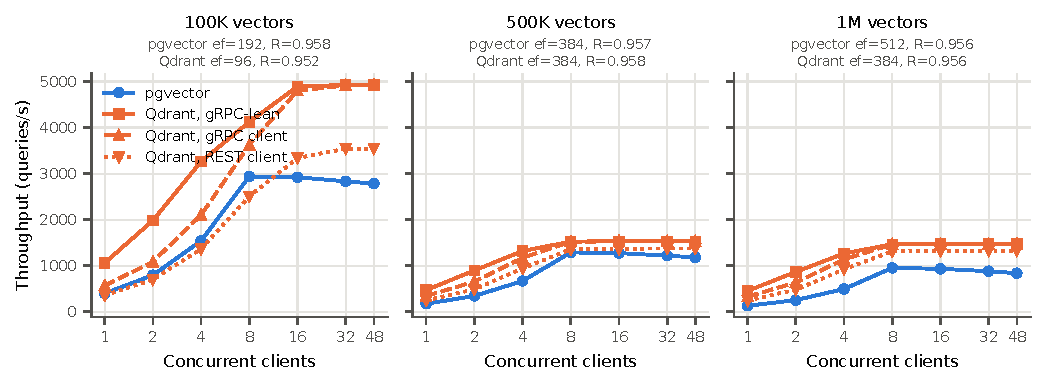
\includegraphics[width=\textwidth]{figures/throughput.pdf}
  \caption{Closed-loop throughput against concurrent client processes at matched recall,
  8 server cores. Panel subtitles give each system's $ef$ and Recall@10.}
  \label{fig:throughput}
\end{figure*}

The two systems behave differently when there are more clients than cores. pgvector
runs one backend process per connection, so 48 clients mean 48 runnable processes on
8 cores. Its throughput drops 5--12\% below the peak, the CPU time per query rises (from
8.3 to 9.5\,ms at 1M), and p99 latency grows to 2.3--3.7$\times$ the mean (130\,ms at
1M). Qdrant queues requests for a fixed pool of search threads. Its throughput stays at
the plateau and its p99 stays within 1.06--1.38$\times$ of the mean (35\,ms at 1M). With
a single client, Qdrant keeps 1.5--2.3 cores busy because it searches its four segments
in parallel. This lowers single-query latency, but it does not raise throughput once all
cores are busy.

\paragraph{Throughput at exactly the matched recall.} The windows above run at the smallest swept $ef$ that reaches the target, so
their recall overshoots it. In the 1M builds of the quantization experiment (Section~\ref{sec:quant}) the overshoot is 0.005 for pgvector and
0.003 for Qdrant at Recall@10 of 0.95, and a higher recall is a slower query. With at least as many clients as cores both engines are CPU bound,
so throughput is inversely proportional to the CPU time of a query. We therefore corrected each build's measured plateau to a recall of exactly 0.95
with its own CPU-per-query curve, interpolated in recall as in Section~\ref{sec:hnsw}:
$\mathrm{qps}(0.95)=\mathrm{qps}(ef_{\mathrm{matched}})\,\mathrm{cpu}(ef_{\mathrm{matched}})/\mathrm{cpu}(0.95)$.
We checked the proportionality against the second $ef$ that each window was run at ($ef=64$): at 32 clients the formula predicts the measured throughput
within 2.7\,\% for pgvector and 3.7\,\% for Qdrant (the largest error over three builds), while for Qdrant at 8 clients the error is up to 15\,\%: at $ef=64$ eight clients keep only 7.1 of the 8 cores busy (7.9 with 32 clients), so that window is not
saturated and the proportionality does not apply. We correct the 32-client plateau only. At 1M the plateau at exactly 0.95 is 13.9\,\% higher for pgvector (1037 instead of 910 queries per
second) and 10.6\,\% higher for Qdrant (1650 instead of 1492), so Qdrant's advantage at the plateau is 1.59 times instead of 1.64 times. At 500K (the 24 builds of
Section~\ref{sec:hnsw}, 24 windows of each engine) the corrections are 6.2\,\% and 6.7\,\%, with prediction errors of $-$0.3\,\% and $-$2.3\,\% on average. The throughput figures above
come from a single build per scale at an overshoot of about 0.006, which is not corrected here because that run did not record CPU per query; by the same
estimate they are about 10 to 14\,\% low. The ratio between the engines moves by about 3\,\%, so no conclusion of this section depends on the correction.

Engine-side times cannot be compared directly between the systems under load. Qdrant's
request time includes the wait for a free search thread, while a PostgreSQL backend
waits in the operating system's run queue before its statement starts, which the
statement time does not include. For this reason we compare engine-side times only at
$C=1$ and use end-to-end latency under load.

Hardware counters measured on the server processes during the 8-client windows give a
view that does not depend on either system's own timing. They count user-space events
only, because the nodes restrict kernel-side counting, and they are normalized by the
queries completed in the window. At matched recall (Recall@10 of 0.95--0.96), pgvector
executes 5.2, 10.0 and 12.7 million instructions per query at 100K, 500K and 1M, and
Qdrant over lean gRPC executes 2.3, 6.8 and 6.7 million, a ratio of 2.2, 1.5 and
1.9$\times$. The cycle ratio is smaller (1.6, 1.2 and 1.5$\times$) because Qdrant runs
at a lower IPC (0.48--0.55 against 0.59--0.75 for pgvector), which is consistent with a
search that spends more time waiting on memory. The client path changes the work done in
the server only for REST. The official gRPC client matches lean gRPC (within 1\% in
instructions per query), whereas REST adds 2.5 million instructions per query at every
scale, 37\% at 500K and 1M and 107\% at 100K, which is the JSON handling that lowers its
plateau above. These counters come from a single build per scale, so we use them to
support the direction and rough size of the differences and not exact ratios.

\subsection{HNSW Parameters}
\label{sec:hnsw}

Table~\ref{tab:hnsw} repeats the 500K comparison with eight construction settings. We
built each configuration three times and interpolated every build's curves to
Recall@10 = 0.95, which removes the earlier dependence on which swept $ef$ happened to
reach the target. In all eight settings Qdrant's single-client latency over lean gRPC is
2.4--3.2$\times$ lower than pgvector's, and its server CPU time per query is
1.3--1.6$\times$ lower. The gap is therefore not specific to $M=16$,
$ef_{construction}=64$, and the latency gap is again larger than the gap in work. Denser
graphs let both systems reach the target at a smaller $ef$. For pgvector they also raise
the build time. Load plus \texttt{CREATE INDEX} grows from 107\,s to 569\,s across the
grid, with a standard deviation of at most 26\,s. Qdrant's total build time stays between
126 and 185\,s, with a standard deviation of up to 76\,s at some settings. Its builds
are dominated by the single-stream upload, so we do not compare them with pgvector's here
(Section~\ref{sec:build}).

\begin{table*}[t]
  \caption{HNSW construction parameters at 500K, three builds per row, each interpolated
  to Recall@10 = 0.95. Latency in ms as seen by the client (mean $\pm$ standard deviation
  across builds), server CPU time per query in ms (mean). Ratios are pgvector divided by
  Qdrant.}
  \label{tab:hnsw}
  \small
  \begin{tabular}{rr|rr|rr|rr}
    \toprule
     & & \multicolumn{2}{c|}{pgvector} & \multicolumn{2}{c|}{Qdrant} & \multicolumn{2}{c}{Ratio} \\
    $M$ & $ef_c$ & latency & CPU & latency & CPU & latency & CPU \\
    \midrule
    16 & 64 & 4.85 $\pm$ 0.11 & 4.76 & 1.73 $\pm$ 0.06 & 3.72 & 2.8 & 1.3 \\
    16 & 128 & 3.14 $\pm$ 0.13 & 3.06 & 1.20 $\pm$ 0.03 & 2.26 & 2.6 & 1.4 \\
    16 & 256 & 2.50 $\pm$ 0.03 & 2.42 & 1.06 $\pm$ 0.02 & 1.88 & 2.4 & 1.3 \\
    32 & 64 & 5.12 $\pm$ 0.06 & 5.03 & 1.79 $\pm$ 0.08 & 3.82 & 2.9 & 1.3 \\
    32 & 128 & 3.63 $\pm$ 0.09 & 3.54 & 1.23 $\pm$ 0.01 & 2.32 & 3.0 & 1.5 \\
    32 & 256 & 2.91 $\pm$ 0.12 & 2.83 & 1.15 $\pm$ 0.03 & 2.11 & 2.5 & 1.3 \\
    64 & 128 & 4.21 $\pm$ 0.18 & 4.12 & 1.31 $\pm$ 0.00 & 2.50 & 3.2 & 1.6 \\
    64 & 256 & 3.60 $\pm$ 0.15 & 3.51 & 1.23 $\pm$ 0.04 & 2.24 & 2.9 & 1.6 \\
    \bottomrule
  \end{tabular}
\end{table*}

Build-to-build variation is small. Across the sixteen engine and setting cells, the
standard deviation of the interpolated latency is 0.2--4.5\% of its mean, and the
standard deviation of Recall@10 at $ef=128$ is at most 0.0025. pgvector's latency still
does not decrease steadily with graph density. The $(32,64)$ graph is slower than
$(16,64)$ by 0.27\,ms and $(64,128)$ is slower than $(32,128)$ by 0.58\,ms, which are 3.6
and 4.9 standard errors of the difference. These gaps are systematic and not variation
between builds, as we had suspected from single builds. We have not isolated their cause.

\textbf{A limit of pgvector's \texttt{ef\_search}.} Our largest swept $ef$ was 1024 for the
E6 and E8 runs, but pgvector accepts \texttt{hnsw.ef\_search} only up to 1000. For a larger
value the server issues a warning and keeps the previous setting (40), without an error.
The pgvector rows at $ef=1024$ in those two experiments were therefore measured at
$ef=40$, and we exclude them. This does not change any reported number: every pgvector
build in E6 and E8 reached Recall@10 = 0.95 at $ef\le 512$, and the matched values are
taken from the smallest such $ef$. The harness now confirms the setting after applying
it. We list this because a benchmark that sweeps $ef$ past 1000 would otherwise measure a
different point than it records.

\subsection{Dimensionality}
\label{sec:dims}

Figure~\ref{fig:dims} varies the dimension from 128 to 1024 at 100K vectors. Qdrant is run
twice at each dimension, once with the default optimizer settings and once with the
indexing threshold lowered to 1\,KB so that every segment gets an HNSW graph. When every
segment is indexed, Qdrant's engine time grows smoothly with $d$, from 0.21 to 0.44\,ms at
$ef=64$, and pgvector's grows from 0.77 to 1.05\,ms. At Recall@10 = 0.90 Qdrant's engine
is 2.9--5.3$\times$ faster across dimensions, and the gap is largest at $d=128$. With the
default settings, Qdrant leaves 1.7--5.8\% of the vectors unindexed at five of the eight
dimensions. This happens whenever the last segment ends up smaller than the 20\,MB
threshold, and those vectors are then scanned exhaustively. At these dimensions the
engine time rises by up to 1.9$\times$ and recall also rises, because part of each answer
comes from an exact scan. The resulting saw-tooth curve is the ``384-dimension anomaly''
we saw in our first measurements. It comes from the optimizer state, and SIMD alignment
does not explain it.

pgvector's recall at $ef=64$ in the single build of this experiment fell to 0.871 at 768
dimensions, 0.013 below its value at 640 and 0.020 below its value at 896. We rebuilt every
dimension three times (E18, Section~\ref{sec:perquery}). At 768 dimensions the three builds
give 0.877 with a standard deviation of 0.001, which is 0.008 below 640 dimensions (0.885) and
0.002 below 896 (0.879). Across all eight dimensions pgvector's recall at $ef=64$ lies between
0.870 and 0.885, with a standard deviation across builds of at most 0.0075. The sharp drop
therefore came mostly from that single build, and a dip of about 0.008 remains at 768
dimensions. We did not find its cause.

\begin{figure*}[t]
  \centering
  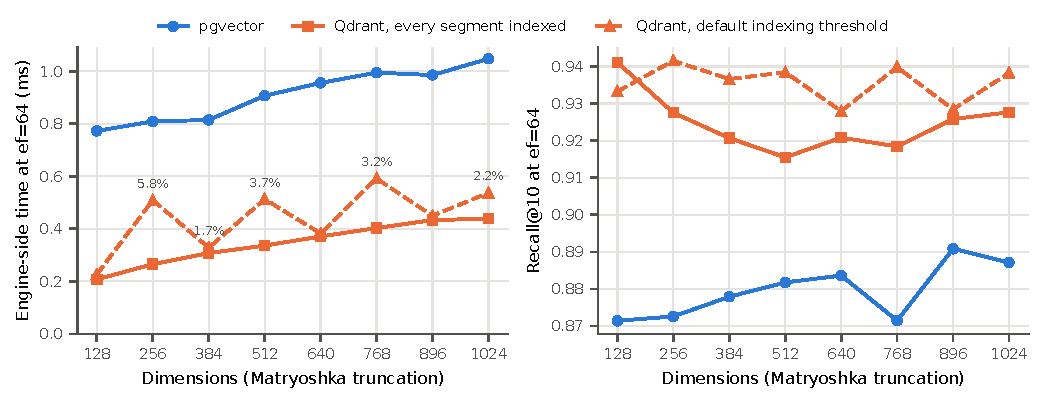
\includegraphics[width=\textwidth]{figures/dimensionality.pdf}
  \caption{Engine-side time (left) and Recall@10 (right) at $ef=64$ against dimension,
  100K vectors. Labels give the share of vectors Qdrant left unindexed with its default
  indexing threshold.}
  \label{fig:dims}
\end{figure*}

\subsection{Memory Pressure}
\label{sec:memory}

\textbf{Buffer pool.} Table~\ref{tab:sb} shows pgvector at 1M vectors with four sizes of
shared buffers. Nothing in these runs is read from disk. The machine has far more memory
than the data, and a page that is not in shared buffers is copied from the operating
system's page cache. Even so, the buffer pool size changes the results considerably.
With 32\,GB the whole index is in shared buffers, every block access is a hit, and the
sampled backends spend all their time on CPU. With the default 128\,MB, 82\% of the
block accesses miss and are read from the page cache, the engine time at $ef=64$ rises
from 1.41 to 3.82\,ms (2.7$\times$), and throughput at $C=8$ falls from 4{,}954 to
1{,}648\,qps (3.0$\times$). At $ef=512$, which reaches Recall@10 = 0.956, the effect is
the same: 7.52 against 20.50\,ms and 978 against 307\,qps.

Each read from the page cache costs about 3\,$\mu$s per 8\,KiB block in every
configuration, and the read time that PostgreSQL records accounts for 86--108\% of the
extra engine time. The copies are also CPU work, which is why throughput falls along
with latency. The server CPU time per query at $C=8$ grows from 1.52\,ms with 32\,GB to
4.68\,ms with 128\,MB. With 32 clients, backends also wait on the buffer mapping lock
(\texttt{LWLock:BufferMapping}, 41\% of samples with 128\,MB), and p99 latency at
$ef=64$ grows from 15.7 to 65.9\,ms. A 4\,GB buffer pool, about half the index, recovers
part of the loss: 77\% of the accesses hit and the engine time is 2.33\,ms.

This confirms, with direct measurement, the buffer-pool explanation that we could only
suggest in our first measurements. It also means that the size of the gap between the
two systems depends on how PostgreSQL is configured. Our main results use 32\,GB of
shared buffers. With PostgreSQL's default, pgvector's engine time would be about
2.7$\times$ longer, and Qdrant's engine advantage at matched recall correspondingly
larger.

\begin{table}[h]
  \caption{pgvector at 1M vectors with different \texttt{shared\_buffers}, no memory limit
  (whole index in the OS page cache). Hit ratio and blocks read per query at $ef=64$;
  engine time (ms) and throughput at $C=8$ (qps) at $ef=64$ (Recall@10 = 0.84) and
  $ef=512$ (0.956).}
  \label{tab:sb}
  \small
  \begin{tabular}{r|rr|rr|rr}
    \toprule
     & & & \multicolumn{2}{c|}{$ef=64$} & \multicolumn{2}{c}{$ef=512$} \\
    shared buffers & hit & reads & eng. & qps & eng. & qps \\
    \midrule
    32\,GB & 1.00 & 0 & 1.41 & 4954 & 7.52 & 978 \\
    4\,GB & 0.77 & 273 & 2.33 & 2456 & 12.99 & 506 \\
    1\,GB & 0.34 & 758 & 3.73 & 1771 & 20.06 & 329 \\
    128\,MB & 0.18 & 939 & 3.82 & 1648 & 20.50 & 307 \\
    \bottomrule
  \end{tabular}
\end{table}

\textbf{Memory limits.} We repeated the memory study with the full query set (E10). For each
system and limit, a fresh server is started with its files evicted from the page cache and
the memory limit applied (including the case without a limit), and one client runs three
passes over all 1{,}677 queries at $ef=128$, each pass in its own random order. The first
pass is the cold start. The later passes are the steady state, and the table reports the
last one. Every configuration was run three times. pgvector is run with 1\,GB of shared
buffers and with shared buffers set to a quarter of the limit, which accounts for the
buffer pool inside the limit (32\,GB when there is no limit). Qdrant memory-maps its
vectors and graph.

The data on disk differs in size. pgvector's index takes 7.61\,GiB, while Qdrant's whole
storage, vectors and graph together, takes 3.94\,GiB. A 1024-dimensional vector fills about
half of an 8\,KiB page, and pgvector stores one graph element per page
(Section~\ref{sec:build}), so it must read and cache about twice as many bytes for the same
vectors in the 32-bit layout (Section~\ref{sec:quant} gives the \texttt{halfvec} and \texttt{int8} variants).

\begin{table*}[t]
  \caption{Cold start and steady state under cgroup memory limits, 1M vectors, $ef=128$,
  all 1{,}677 queries per pass, one client, spinning disk. Mean latency per query in ms,
  mean of three repetitions; ``cold'' is the first pass after a restart with an evicted page
  cache and ``steady'' the last of the next two passes. pgvector with 1\,GB of shared
  buffers, and with shared buffers equal to a quarter of the limit (32\,GB without a limit).
  The Qdrant 4\,GB steady values are listed per repetition because they differ in kind.
  pgvector at 4\,GB did not finish within the 3\,h job limit (Section~\ref{sec:memory}).}
  \label{tab:caps}
  \small
  \begin{tabular}{r|rr|rr|rr}
    \toprule
     & \multicolumn{2}{c|}{pgvector, 1\,GB buffers} & \multicolumn{2}{c|}{pgvector, buffers = limit/4}
     & \multicolumn{2}{c}{Qdrant} \\
    limit & cold & steady & cold & steady & cold & steady \\
    \midrule
    none & 1132 & 6.56 & 972 & 2.29 & 611 & 1.19 \\
    16\,GB & 1065 & 6.52 & 1051 & 4.21 & 656 & 1.24 \\
    8\,GB & 1246 & 636 & 1503 & 1171 & 570 & 1.22 \\
    4\,GB & \multicolumn{2}{c|}{not finished} & \multicolumn{2}{c|}{not finished} & 766 & 1.20, 1.43, 34.6 \\
    \bottomrule
  \end{tabular}
\end{table*}

Table~\ref{tab:caps} gives the results. The cold start is slow for both systems, because each query waits for random reads from the
spinning disk: 1.0--1.5\,s per query for pgvector and 0.6--0.8\,s for Qdrant, or 0.3 to
0.7 hours for the 1{,}677 queries. The steady state then separates the systems. Qdrant's
latency is 1.2\,ms with no limit, with 16\,GB and with 8\,GB, which is the same as without
a limit. pgvector is close to its in-memory latency at 16\,GB (6.5\,ms with 1\,GB of
buffers, 4.2\,ms when the buffers take a quarter of the limit) but at 8\,GB it is at
636\,ms and 1{,}171\,ms per query, or 1.6 and 0.9 queries per second, because its 7.6\,GiB
index no longer fits. Giving the buffer pool a quarter of the limit did not help at 8\,GB.

The earlier version of this study used 300 queries, one repetition and a fixed window
order, and concluded that pgvector was back to 3.6\,ms with 8\,GB. With the full query set
pgvector is at 636\,ms for the same limit. The difference in $ef$ between the studies (64
and 128) cannot explain a factor of 100. The 300 queries touched only part of the graph,
and that part fitted, as the referee suspected.

At 4\,GB, Qdrant's data (3.9\,GB resident) is just below the limit (4.29\,GB), and its
behavior differs between repetitions. In one repetition the second pass was already at
1.2\,ms, in another it needed two passes to reach 1.4\,ms, and in the third it was still at
35\,ms after two steady passes, with 17{,}800 major page faults in the last one. The
8-client throughput measured after the passes was 3{,}395, 3{,}351 and 299\,qps. We
therefore do not report a single latency for Qdrant at this limit: it returns to its
in-memory latency in two of three repetitions, and not within two passes in the third.
pgvector did not complete three passes at 4\,GB within the 3\,h limit of a job. We did not
repeat these runs with a longer limit.

Without a limit, Qdrant's memory-mapped files were also not in the page cache after
the restart, so its first pass was as slow as under the limits. The buffer pool effect
reappears in the rows without a limit: pgvector with 1\,GB of buffers needs 6.56\,ms per
query at steady state and 152\,qps, against 2.29\,ms and 435\,qps with 32\,GB, a ratio of
2.9$\times$ for the same data in the same page cache.

%% =============================================================
\subsection{Quantization}
\label{sec:quant}

The index sizes above are for 32-bit floats. We repeated the 1M build with each system's own
reduced-precision storage: pgvector with a \texttt{halfvec} column and \texttt{halfvec\_cosine\_ops}
index (16-bit floats), and Qdrant with scalar \texttt{int8} quantization (quantized vectors kept in
RAM, candidates rescored with the original vectors, Qdrant's default oversampling). Each system
was built three times, and each job built both arms of one system, one after the other on one node.
The two systems ran on different nodes (Table~\ref{tab:sources}). Recall is measured against the exact
32-bit neighbors, so a recall below the float arm is the accuracy lost to quantization.
Table~\ref{tab:quant} gives the results; the ratios below are paired within a build
(mean of three, with 95\% intervals).

\begin{table}[t]
  \caption{Float against reduced precision, 1M vectors, 1024 dimensions, three builds each.
  Latency and CPU are interpolated in recall to 0.95. Size is the pgvector index, then the
  whole table with TOAST and index; for Qdrant it is the storage directory at the end of the
  build (range over the three builds). The Qdrant float size varies between builds for a
  reason we did not find.}
  \label{tab:quant}
  \small
  \begin{tabular}{@{}lrrrrr@{}}
    \toprule
    & \multicolumn{2}{c}{size (GiB)} & build & latency & CPU \\
    arm & index & total & s & ms & ms/query \\
    \midrule
    pgvector \texttt{vector} & 7.61 & 12.84 & 273 $\pm$ 15 & 6.73 $\pm$ 0.15 & 6.64 \\
    pgvector \texttt{halfvec} & 2.54 & 5.20 & 160 $\pm$ 4 & 6.28 $\pm$ 0.43 & 6.19 \\
    Qdrant float32 & \multicolumn{2}{c}{3.93--5.24} & 343 $\pm$ 54 & 2.00 $\pm$ 0.02 & 4.49 \\
    Qdrant \texttt{int8} & \multicolumn{2}{c}{4.89--6.49} & 365 $\pm$ 39 & 1.26 $\pm$ 0.04 & 2.47 \\
    \bottomrule
  \end{tabular}
\end{table}

\paragraph{pgvector \texttt{halfvec}.} The index is 0.334 times as large (2.54 against 7.61\,GiB)
and the table with its TOAST data 0.405 times (5.20 against 12.84\,GiB). The build takes 0.59
times as long (0.49 to 0.68). Search speed at matched recall does not change measurably: the
latency ratio is 0.93 (0.73 to 1.13) and the CPU ratio 0.93 (0.73 to 1.14), at $ef$ of 455 and 439. Closed-loop throughput at the
matched $ef$ (512 for both) is 1.09 to 1.10 times higher (intervals 1.06 to 1.14) at one, eight and 32 clients, and
at the fixed $ef=64$ it is not distinguishable from 1 for one and eight clients (1.02, 0.96 to 1.07; 1.02, 0.97 to 1.07) and borderline at 32 (1.04, 1.00 to 1.08).
We did not find
why half the vector bytes do not shorten the search. Recall does not drop: the highest recall on
the grid differs by $-0.0009$ ($-0.007$ to $0.005$) and the share of queries with recall below 0.8 by
$-0.0006$ ($-0.014$ to $0.012$).

\paragraph{Qdrant \texttt{int8}.} Latency at matched recall is 0.63 times that of the float
arm (0.57 to 0.69; $p99$ 0.60, 0.54 to 0.66), server CPU per query 0.55 times (0.48 to 0.62), and closed-loop throughput 1.67, 1.91 and 1.92
times at one, eight and 32 clients at the matched $ef$ (338 and 339 on average, the
interpolated $ef$ ratio is 1.01, 0.84 to 1.18), and 1.33 to 1.59 times at $ef=64$. Quantization costs
little recall. The highest recall on the grid differs by $-0.0024$ ($-0.009$ to $0.004$). The share
of queries that find all ten neighbors, however, falls by 0.025 (0.014 to 0.035) at the same mean
recall, so the loss is spread over many queries. Build time does not change (1.07, 0.93 to 1.21). The
storage directory is not smaller, since the original vectors stay on disk for rescoring and the
quantized copy is added: 5.3 to 7.0\,GB against 4.2 to 5.6\,GB. The quantized copy adds about
1\,GB (one byte per dimension and vector), which the build-to-build variation of the storage size hides,
so we do not report a ratio.

\paragraph{The size comparison.} Section~\ref{sec:memory} compares pgvector's 7.61\,GiB index with
Qdrant's 3.94\,GiB of storage and concludes that pgvector has to cache about twice as many bytes. With three
builds, Qdrant's float32 storage is 3.93 to 5.24\,GiB, so the index of the float layout is 1.5 to 1.9
times its size and the whole pgvector table 2.4 to 3.3 times. With \texttt{halfvec} the index shrinks to 0.48 to 0.65
times Qdrant's float32 storage, and the whole table to 1.0 to 1.3 times. The ``twice as large'' statement is therefore a
property of the 32-bit layout (one graph element per 8\,KiB page, Section~\ref{sec:build}), not of
pgvector at 1024 dimensions in general.

\subsection{Ranking Quality}
\label{sec:ranking}

Recall@10 counts the neighbors that exact search would return. It does not say whether the lost neighbors would have
mattered to a user. Relevance judgments exist for the TREC Deep Learning queries, so we asked how much ranking quality
approximate search loses. The question has a limit that decides what can be claimed. Our corpus is the first million
rows of the MS MARCO v2.1 segment stream, about 0.9\,\% of the collection the judgments were made against. We fixed a
rule before looking (the repository file \texttt{docs/E23\_GATE.md}): absolute nDCG only if at least half of the
relevant documents are in the corpus, a sensitivity analysis if at least 50 queries still have one.

\paragraph{Coverage.} The judgments name v2 documents (2021 and 2022) or v2 passages (2023), while the stream
holds v2.1 segments, and the numbers inside the two kinds of identifier are byte offsets in different files (the second
document is 4806 in v2 and 4810 in v2.1). Comparing the identifiers, as we first did, finds no judged document
in the corpus; that zero is a failed match, not a coverage. We matched documents by URL instead: all 105{,}546 documents of the corpus
have exactly one v2 document with the same URL. Of 53{,}761 relevant documents (grade 2 or 3) of 214 judged queries, 385 are in
the corpus, a coverage of 0.72\,\%, and 63 queries (25, 17 and 21 of the years 2021, 2022 and 2023) have at least one. The
coverage is far below one half and the query count is above 50, so the rule allows a sensitivity analysis only.

\paragraph{Setup.} We score those 63 queries. A segment takes the grade of its document, nDCG@10 uses the grades
as gains, and the ideal ranking is the best ten segments the corpus holds, so a query is scored on what the corpus can
contain. MRR@10 and Recall@10 count grades 2 and 3 as relevant. The reference is the exact top ten of the same corpus.
For each engine we built the index 3 times (1M vectors, 1024 dimensions, $M=16$, $ef_{construction}=64$) and kept the
returned identifiers at ten $ef$ values; the numbers are means over builds, and the intervals are bootstrap intervals over
queries. Table~\ref{tab:ranking} gives the exact result and each engine at $ef=64$ and at the smallest swept $ef$ whose
recall against the exact neighbors reaches 0.95.

\begin{table}[t]
  \caption{Ranking quality of approximate search against exact search on the same 1M corpus (sensitivity analysis,
  63 queries with a relevant document in the corpus). Recall is against the exact neighbors over all 1{,}677 queries.
  Ratios are the engine's value divided by the exact value; the interval is for the mean per-query difference in nDCG@10.}
  \label{tab:ranking}
  \small
  \begin{tabular}{@{}lrrrrrrr@{}}
    \toprule
    & $ef$ & recall & nDCG@10 & ratio & difference to exact & MRR ratio & R@10 ratio \\
    \midrule
    exact & -- & 1.000 & 0.388 & 1.000 & -- & 1.000 & 1.000 \\
    pgvector & 64 & 0.836 & 0.366 & 0.942 & -0.062 to +0.004 & 0.923 & 0.947 \\
    pgvector, matched & 512 & 0.955 & 0.380 & 0.979 & -0.026 to +0.002 & 0.960 & 0.987 \\
    Qdrant & 64 & 0.861 & 0.371 & 0.955 & -0.039 to -0.002 & 0.925 & 0.961 \\
    Qdrant, matched & 384 & 0.954 & 0.382 & 0.984 & -0.023 to +0.004 & 0.966 & 0.994 \\
    \bottomrule
  \end{tabular}
\end{table}

\paragraph{Result.} The exact top ten has nDCG@10 of 0.388 (95\,\% interval 0.306 to 0.472 over the queries), MRR@10 of 0.489 and
Recall@10 of 0.364 on this corpus; these are not effectiveness numbers, because 99.3\,\% of the relevant documents are
outside it.
At the smallest swept $ef$ reaching a recall of 0.95 against the exact neighbors, pgvector (at $ef=512$) keeps 97.9\,\% of
the exact nDCG@10 and Qdrant (at $ef=384$) 98.4\,\%. The 95\,\% intervals of the mean difference to exact search, -0.026 to +0.002 and -0.023 to +0.004, both contain
zero, so at this recall neither engine is distinguishable from exact search on these queries. MRR@10 keeps 96.0\,\% and
96.6\,\%, Recall@10 98.7\,\% and 99.4\,\%.

\paragraph{Relation to recall.} Over the 20 swept points the nDCG@10 ratio is higher than the recall of the same 63 queries in 19 of them (the
table's recall column is over all 1{,}677 queries and is lower). A missed neighbor therefore usually costs less ranking
quality than its share of the ten suggests. At $ef=32$, with recalls of 0.76 and 0.79, the engines keep 90\,\% and 92\,\% of the exact nDCG@10 and the interval of the
difference excludes zero; across the grid the interval lies entirely below zero at 6 of 20 points, all at or below $ef=256$.

\paragraph{What this does and does not show.} Only 63 queries, uneven over the years, and a relevance
signal taken from documents and copied to their segments. The ratios describe how much ranking quality an approximation
at a given recall costs on a corpus that holds a small part of the relevant documents; they do not rank the two systems by
effectiveness, which would need a corpus that holds the judged documents. Extending to the full collection of 113 million
segments is outside this study.


\subsection{Connection Pooling}
\label{sec:pooling}

A common recommendation for PostgreSQL with more clients than cores is to put a connection pooler in front of it. We tested
it for pgvector. The pooler is PgBouncer 1.25.1 from the project's container image, pulled by digest (the digest and the
image checksum are in the run record), in transaction pooling mode with a pool of 8 server connections, equal to the 8 cores of the server, and
pinned to those same cores, so that its CPU time competes with PostgreSQL's and is counted in the server CPU per query. The
index is the 1M $\times$ 1024 index of the other experiments, built 3 times. Each build serves three connection modes one
after the other, so a comparison is within a build: \emph{direct}, the baseline of the rest of this paper (one session, settings
made once with \texttt{SET}); \emph{transaction}, where every query is a transaction of its own that starts with
\texttt{SET LOCAL hnsw.ef\_search} and \texttt{SET LOCAL enable\_seqscan}, without a pooler; and \emph{PgBouncer}, the same
transactions through the pooler. The transaction arm exists because a transaction pooler does not keep session settings: the
next statement may reach another server connection, and a session-level \texttt{SET} would silently run the query at the wrong
$ef$. It separates the cost of the per-query transaction from the cost of the pooler. We ran closed-loop windows of 30\,s with 1,
8, 32 and 48 clients at $ef=448$, the smallest swept value with Recall@10 of 0.95 on every build, and at $ef=64$. Recall
in the three modes agrees ($0.951$ to $0.952$ at $ef=448$), which shows that the settings reached the queries.

\begin{table}[t]
  \caption{pgvector at $ef=448$ (Recall@10 about 0.95), 1M vectors, mean of 3 builds. CPU is server CPU per query in ms,
  including the pooler. Active is the mean number of backends working at a sample of the wait-event sampler.}
  \label{tab:pooling}
  \small
  \begin{tabular}{@{}rlrrrrr@{}}
    \toprule
    clients & mode & qps & mean ms & p99 ms & CPU & active \\
    \midrule
    1 & direct & 151 & 6.6 & 10.1 & 6.53 & 1.0 \\
     & transaction & 145 & 6.9 & 10.3 & 6.66 & 1.0 \\
     & PgBouncer & 147 & 6.8 & 10.3 & 6.58 & 0.9 \\
    \addlinespace
    8 & direct & 1125 & 7.1 & 10.9 & 7.00 & 7.9 \\
     & transaction & 1092 & 7.3 & 11.1 & 7.07 & 7.6 \\
     & PgBouncer & 1065 & 7.5 & 12.3 & 7.09 & 7.4 \\
    \addlinespace
    32 & direct & 1052 & 30.4 & 76.4 & 7.56 & 21.3 \\
     & transaction & 1038 & 30.8 & 52.8 & 7.65 & 15.6 \\
     & PgBouncer & 1058 & 30.2 & 36.7 & 7.09 & 7.3 \\
    \addlinespace
    48 & direct & 1014 & 47.3 & 131.0 & 7.85 & 35.6 \\
     & transaction & 998 & 48.1 & 99.2 & 7.96 & 25.6 \\
     & PgBouncer & 1059 & 45.3 & 52.0 & 7.09 & 7.4 \\
    \bottomrule
  \end{tabular}
\end{table}

\paragraph{With fewer clients than cores the pooler does not help.} With one client the throughput through the pooler is 0.97 (0.92 to 1.02)
times the direct one, which is not distinguishable from 1, and with eight clients 0.95 (0.93 to 0.97) (ratios of the same build, mean of three, 95\,\% interval). The pooler
uses 0.088\,ms of CPU per query at eight clients, 1.2\,\% of the server CPU per query, and 0.09 of a core; at 32 and 48
clients it uses 0.10 and 0.10 of a core, so a single-threaded pooler is far from its own limit. The per-query
transaction accounts for part of the loss (throughput 0.96 (0.94 to 0.98) and 0.97 (0.97 to 0.97) of direct at one and eight clients).

\paragraph{With more clients than cores it cuts the tail, not the throughput.} At 32 and 48 clients, throughput through the pooler is
1.01 (0.97 to 1.04) and 1.04 (1.01 to 1.08) times the direct one, so the plateau of about 1{,}050 queries per second is the server's and
hardly moves. Mean latency is 0.99 (0.96 to 1.03) and 0.96 (0.92 to 0.99) times the direct one, and p99 latency is 0.48 (0.44 to 0.52) and 0.42 (0.12 to 0.73)
times, from 76 to 37\,ms at 32 clients and from 131 to 52\,ms at 48. The direct p99
at 48 clients is unstable across builds (standard deviation 40\,ms), which is why its interval is wide. Server CPU per query,
with the pooler's share included, is 0.94 (0.93 to 0.94) and 0.90 (0.88 to 0.93) times the direct one. The wait-event sampler shows what changes:
with direct connections 21 and 36 backends are active on average at 32 and 48 clients, with the
pooler 7.3 and 7.4. The lock manager takes 0.09\,\% and 0.22\,\% of the active-backend observations in the direct
runs and none behind the pooler, which is too little to explain the CPU difference; we did not isolate its cause. Voluntary context
switches per query rise from 1.1 (direct) to 5.1 (transaction) and 12.9 (pooler) at 48 clients, so the pooler adds wake-ups
and does not save scheduler work.

\paragraph{Part of the tail effect is the per-query transaction.} Comparing the transaction arm with the direct one, p99 at 32 and
48 clients is 0.69 (0.60 to 0.79) and 0.82 (0.05 to 1.58) times the direct value; the pooler lowers it by a further 0.69 (0.63 to 0.76) and 0.53 (0.42 to 0.64)
times, and throughput through the pooler is 1.02 (0.98 to 1.06) and 1.06 (1.06 to 1.07) times that of the transaction arm. The tail
improvement of the pooler alone is therefore smaller than the figures against direct connections suggest, and at 48 clients the
interval of the transaction arm is too wide to apportion it.

\paragraph{With short queries the overhead weighs more.} At $ef=64$ (recall 0.84), where a query is short, the throughput
through the pooler is 0.75 to 0.83 times the direct throughput across the four client counts: this
fits a fixed cost per query, from the extra statements and the extra hop, that weighs more when the query is short; we did not isolate it.

\paragraph{Reading.} For this workload, a pooler with a pool equal to the number of cores is a tail-latency control, not a
throughput gain. When clients outnumber cores it brings p99 latency to 0.48 (0.44 to 0.52) and 0.42 (0.12 to 0.73) times that of direct connections
at 32 and 48 clients (0.69 (0.63 to 0.76) and 0.53 (0.42 to 0.64) times that of the same transactions without a pooler), costs about
0.091\,ms of CPU per query, and costs throughput when the system is not saturated or the queries are short. Using it also changes how the index must be configured, since
settings have to travel with each transaction. We did not test other pool sizes, session pooling, a pooler on separate cores
or a separate host (the pooler here is on the loopback interface and on the server's cores), open-loop load or other clients.


\subsection{Open-Loop Load}
\label{sec:openloop}

The concurrency results above are closed loop: a client sends its next query when the last one returns, so a server that slows
down also slows the load. Real traffic arrives whether or not the server keeps up. We therefore sent Poisson arrivals at fixed rates,
and measured latency from the planned send time, so that a server that falls behind shows its queue as latency. The load levels are
fractions of each build's own closed-loop throughput at 32 clients at its matched-recall $ef$ ($ef=448$ and a mean of $363$ for
pgvector and Qdrant; capacity 1{,}028 and 1{,}566 queries per second), so the two engines are compared at the same relative load and
not at the same absolute rate. A level is a window of 90\,s after the connections have been made and warmed up; the first 30\,s are a ramp at the
target rate and are left out of every statistic. 3 builds per engine, 1M $\times$ 1024, 64 client processes (which bounds the
queries in flight at 64). A level is \emph{settled} if at least 98\,\% of the measured queries finish inside the window and the median
latency of the last quarter of the measured part is within a factor of two (plus 10\,ms) of that of the first quarter in both directions. The
rule, its history and the data it was fixed on are in \texttt{docs/E22\_DESIGN.md}; we state in the next paragraphs where it changed.

\begin{table}[t]
  \caption{Poisson arrivals at fractions of the closed-loop capacity of each build, mean of 3 builds. Done is the
  share of the queries planned in the measured part that finished before the window ended. Latency is given only for settled levels.}
  \label{tab:openloop}
  \small
  \begin{tabular}{@{}llrrlrrr@{}}
    \toprule
    & load & qps & done & settled & mean ms & p99 ms & p99.9 ms \\
    \midrule
    pgvector & 50\,\% & 514 & 100\,\% & yes & 8.1 & 16.2 & 22.8 \\
     & 80\,\% & 823 & 100\,\% & yes & 11.9 & 54.5 & 86.8 \\
     & 95\,\% & 977 & 100\,\% & no & \multicolumn{3}{c}{not a steady state} \\
     & 110\,\% & 1131 & 79\,\% & overload & \multicolumn{3}{c}{not a steady state} \\
    \addlinespace
    Qdrant & 50\,\% & 783 & 100\,\% & yes & 3.0 & 7.4 & 11.2 \\
     & 80\,\% & 1253 & 100\,\% & yes & 5.5 & 25.7 & 36.1 \\
     & 95\,\% & 1488 & 100\,\% & yes & 8.6 & 30.2 & 45.3 \\
     & 110\,\% & 1723 & 86\,\% & overload & \multicolumn{3}{c}{not a steady state} \\
    \bottomrule
  \end{tabular}
\end{table}

\paragraph{Where both systems are settled, pgvector's tail is wider.} At 50\,\% of capacity the p99 latency is 16.2\,ms for pgvector and
7.4\,ms for Qdrant. At 80\,\% (823 and 1253 queries per second, so pgvector is at a lower absolute rate) it is 54.5
and 25.7\,ms, a factor of 2.1, and the p99.9 latency is 86.8 and 36.1\,ms. Server CPU per query is
7.9 and 5.1\,ms at that load, the pattern of the closed-loop measurements (Section~\ref{sec:cpu}). Qdrant is still settled at
95\,\%, with a p99 of 30.2\,ms and a p99.9 of 45.3\,ms.

\paragraph{The closed loop shows a different tail.} The closed-loop p99 at 32 clients is 71.1\,ms for pgvector and 22.4\,ms for Qdrant. A closed loop bounds the
queue at the number of clients and an open loop does not. For Qdrant the open-loop p99 at the highest settled level, 95\,\%, is 1.35 times the closed-loop value, so
although the closed loop keeps the server saturated, its tail is the smaller one. For pgvector the open-loop p99 at its highest settled level, 80\,\%, is
0.77 times the closed-loop value, which is not a contradiction: its 95\,\% level did not settle (next paragraph), so the highest level we can compare is a lighter one than for Qdrant.
The closed-loop tail of Section~\ref{sec:concurrency} should be read as that of a server held at saturation by a fixed number of clients, not as the tail at a given load.

\paragraph{pgvector did not settle at 95\,\%.} The first reading of the data labelled this level steady, because the rule then asked only that latency
not grow. The median latency in the first quarter of the measured part is 656\,ms and in the last quarter 36\,ms:
a backlog that built up during the ramp was still draining throughout the window (mean 574\,ms, p99 4.0\,s over the whole measured part).
With 5\,\% spare capacity a backlog of a second takes a long time to go. We therefore added the second direction to the rule (after seeing these
data, which is why it is described here) and do not give a tail for this level. What it does show is slow recovery: at 95\,\% load pgvector had not returned to the median latency of its 80\,\% level
(9\,ms) by the end of the 90\,s window, while Qdrant's windows at the same relative load carried no backlog. The backlog builds in the first
seconds of a window (a first run with 60\,s windows and a 5\,s ramp showed it already at 80\,\%, and is kept as a record in the repository).
Our reading is that new PostgreSQL backends are slow for their first queries; we did not establish why, and a deployment with long-lived connections
may not see it, as the closed-loop windows of the other experiments, whose backends have been running for a long time, do not.

\paragraph{Beyond capacity.} At 110\,\% neither engine settles, as expected. Of the queries planned in the measured part, 79\,\% (pgvector) and 86\,\% (Qdrant)
finished before the window ended, and the median latency grows from 7.0\,s to 12.9\,s and from 3.8\,s to 8.2\,s over the
measured part. Those numbers depend on the length of the window and carry no tail claim.

\paragraph{Limits.} One $ef$ per build, one query mix, Poisson arrivals only, at most 64 queries in flight, a client on the other socket of the same node, 90\,s windows. The
engines ran on different nodes. We did not vary the number of cores, and we did not test long-lived connections that had been warmed for minutes before the window.


\section{Discussion}
%% =============================================================

\subsection{What the Measurements Say About the Choice}

When the working set fits in memory, Qdrant's single-client latency is 3--4$\times$ lower
than pgvector's at equal recall, from 100K to 1M vectors and for every HNSW configuration
and dimension we tested. Much of this comes from searching segments in parallel: its CPU
time per query is lower by a smaller factor, about 1.4$\times$ with the default four
segments and about equal with eight (Section~\ref{sec:cpu}). The decomposition of
Section~\ref{sec:causal} locates the remaining CPU gap. pgvector does not compute more distances; it reads fewer
vectors per query than Qdrant, but each read costs it about 2.3 times the cycles, and about half of its cycles
are spent outside distance computation and element loading, in the buffer manager and in visited-set and heap bookkeeping, for which Qdrant's profile shows little. For an application, however, the client matters about as much as the engine. Through
Qdrant's official REST client, pgvector was the faster system at Recall@10 = 0.90 at every scale we
measured. A team choosing between the two should therefore consider which client and
protocol it will use, and not only which engine is faster.

Under load, both systems are limited by CPU and not by locking, and they differ in how they handle overload. With a
fixed number of clients, Qdrant's thread pool keeps latency predictable when there are more clients than cores, while
pgvector's process-per-connection model loses some throughput and develops a long latency tail. With Poisson arrivals the
difference shows already at 80\,\% of each system's capacity, where pgvector's p99 latency is about twice Qdrant's, and at
95\,\% pgvector did not settle within the 90\,s window (Section~\ref{sec:openloop}). A connection pooler with a pool equal to
the cores brings pgvector's p99 under overload to about half, but throughput does not rise and below saturation
the pooler costs a few per cent (Section~\ref{sec:pooling}); it also requires that the index settings travel with every
transaction. Build time depends on how each system is loaded. Against Qdrant's single-stream upload, pgvector with its build
parallelism configured built faster, but with parallel streams and deferred indexing Qdrant is
1.4$\times$ faster at 1M, and pgvector's own load is limited by write-ahead logging on this
disk (Section~\ref{sec:ingest}). Build times also varied considerably between nodes, so
single build measurements on a shared cluster should be treated with care.

Memory and precision matter as much as the choice of system. With PostgreSQL's
default buffer pool, pgvector reads most index pages from the operating system's page
cache, and this alone made it 2.7$\times$ slower in our runs, with no disk access at all.
Anyone deploying pgvector, or benchmarking it, should size \texttt{shared\_buffers} to
hold the HNSW index. When the index does not fit in memory at all, pgvector is at a
disadvantage at 1024 dimensions in its 32-bit layout, which needs 1.5 to 1.9 times the bytes of Qdrant's storage for the index alone; storing the vectors in half precision
(\texttt{halfvec}) shrinks the index to a third without a detectable loss of speed or recall, and its index is then 0.5 to 0.65 times Qdrant's 32-bit storage
(Section~\ref{sec:quant}). Qdrant's \texttt{int8} quantization is a speed feature, not a space one: it made a query 1.6 times faster at the same recall, but the original vectors stay on disk
and the storage grew. On our spinning disks a cold query took 0.6 to 1.5
seconds, so neither system is usable out of core on such hardware. Once the data had been
read, Qdrant stayed at its in-memory latency down to a limit of 8\,GB, where pgvector needed
hundreds of milliseconds per query. At 4\,GB, just below the size of Qdrant's data, Qdrant
returned to its in-memory latency in two of three repetitions, and pgvector did not finish.
Finally, a recall of 0.95 is a good proxy for ranking quality in our corpus: on the judged queries that the corpus can answer,
approximate search at that recall keeps 98\,\% of the nDCG@10 of exact search for both engines (Section~\ref{sec:ranking}); the analysis is a sensitivity analysis and says nothing about absolute effectiveness.

\subsection{How Vector Search Benchmarks Go Wrong}

The confounders in Table~\ref{tab:confounders} reversed all three main
results of our first measurements, and Table~\ref{tab:checklist} turns them into a checklist. The later experiments added lessons of the same kind, each of which we met by
getting it wrong first:
\begin{itemize}
  \item \emph{A setting that does not reach the query.} pgvector ignores an \texttt{ef\_search} above 1000 with a warning and keeps its default of 40, and
    a session-level \texttt{SET} does not survive a transaction pooler. A benchmark should read the setting back inside the connection that runs the query.
  \item \emph{The plan, not only the result.} pgvector can stop using the HNSW index for TOASTed vectors without any warning, and the query still returns correct results, only much more slowly.
    Benchmarks, and applications in production, should check the query plan rather than assume the index is used.
  \item \emph{A closed loop hides the queue.} Fixed numbers of clients bound the queue; arrivals at a fixed rate do not, and the first seconds of a window can show a start-up backlog of fresh connections
    that a longer-lived deployment would not see. We had to lengthen the window and add a ramp, and to say after seeing the data that the first criterion for a steady level was too weak.
  \item \emph{An ID is not an ID.} Document numbers of two versions of the same collection are byte offsets in different files. Comparing them found no relevant document in the corpus, which looked like a coverage of zero.
    Matching by URL showed that the corpus holds 0.7\,\% of the judged-relevant documents.
  \item \emph{A metric needs a corpus that can answer it.} Absolute nDCG on a prefix of a collection says little about retrieval effectiveness. We fixed the rule for what could be reported before measuring the coverage.
  \item \emph{Sizes need the same accounting.} The size of Qdrant's storage varied by about a third between builds of the same configuration for a reason we did not find, and a quantized copy adds to it. A ratio of sizes needs the data to be stable
    before it is reported.
  \item \emph{A measurement can disappear with its process.} The CPU time of a PostgreSQL backend that has exited is no longer visible; a harness that reads CPU after its clients have left reports almost nothing for pgvector.
\end{itemize}
Each of these was found by a check that the harness or the analysis now performs, and the checks are in the repository with their tests.

\subsection{Threats to Validity}
\label{sec:threats}

\textbf{Single node, single client language.} Both systems run on a single node and are
queried from Python. Clients written in compiled languages would reduce the client's
share of latency further, and gRPC-lean gives an approximate lower bound for it.

\textbf{Shared infrastructure.} Each node runs only our job, but the parallel file
system and the interconnect are shared with other users. Database files are kept on
node-local disk, and every result records the node's load and any other jobs on it.
Query measurements run from memory and are not affected by the disk, but build times
are, so all build times we report compare configurations on one node. The disk is
rotational, and Section~\ref{sec:ingest} shows that pgvector's load is limited by writing
its log to it, so build times on SSDs may differ.

\textbf{Configuration.} We tune PostgreSQL's memory settings for an in-memory working
set and leave Qdrant at its defaults, apart from $ef_{construction}$. Experiments E2 and
E4 vary the parameters most likely to change the conclusions. E4 shows that with
PostgreSQL's default \texttt{shared\_buffers}, pgvector would compare considerably worse
than in our main results.

\textbf{Memory-limit runs.} The memory-limit runs use a spinning disk, one client, one
value of $ef$ (128) and three repetitions, with the cold start and the steady state
reported separately. They do not show performance on SSDs, where a random read takes a
small fraction of the 4.8\,ms we measured, and the cold start would be much shorter. The
pgvector arms at 4\,GB did not finish within the 3\,h job limit and we did not repeat
them with a longer one, so the comparison at that limit is incomplete. Qdrant's data is
just below the 4\,GB limit, and its three repetitions did not agree, so three
repetitions are not enough to characterize that point. pgvector's shared buffers count
against its memory limit, while Qdrant has no equivalent fixed allocation; the arm with
shared buffers set to a quarter of the limit tests this, and did not help at 8\,GB.

\textbf{Single embedding model and corpus.} All experiments use Cohere v3 embeddings of
MS MARCO. Prefix truncation of a model that was, to our knowledge, not trained for it is
only a rough stand-in for models that natively produce lower-dimensional embeddings, so
the dimensionality results describe index behavior on truncated vectors and do not carry
over to native 384- or 768-dimensional models.

\textbf{Storage.} The nodes we used have a single rotational disk and no NVMe device (checked on four nodes of three partitions, Section~\ref{sec:env}); every result that depends on storage is a worst case. The \texttt{orfoz} partition has NVMe (one node checked) but a different processor, so a repetition there would be a separate platform and is not part of this paper's results.

\textbf{Different nodes for the two systems.} Within an experiment the two systems usually ran on different nodes (Table~\ref{tab:sources}), and the closed-loop and open-loop comparisons between them compare ratios of means over three builds, not paired runs. Within one system, comparisons of arms (precision, connection mode) are paired on one node.

\textbf{Ranking quality.} The nDCG analysis covers 63 queries that have a relevant document in a corpus holding 0.7\,\% of the judged-relevant documents, grades are copied from documents to their segments, and the numbers are ratios to exact search, not effectiveness. The 2023 judgments were linked to documents through passage identifiers of the earlier collection version.

\textbf{Open-loop load.} The first run of the open-loop experiment (60\,s windows) showed a start-up backlog for pgvector; the second (90\,s windows with a 30\,s ramp) changed the rule for a settled level after its data were seen. Both runs are in the repository, and the rule and its history are in the design note. We did not test connections that had been warmed for minutes.

\textbf{Reduced precision.} One embedding model, one dimension, one quantization setting per engine (\texttt{halfvec}; \texttt{int8} with rescoring and Qdrant's default oversampling). Qdrant's storage size varied between builds, so we report ranges and no size ratio for \texttt{int8}.

\textbf{Provenance.} The first experiments (E1--E5) were archived before the provenance system existed and have no commit or seed in their files. The numbers in the prose of the sections that are not written from analysis files were copied from the analysis summaries by hand; the analysis files are regenerated and checked, only the headline numbers and the cells of the result tables are recomputed (Section~\ref{sec:provenance}).

\textbf{Engine-side timing.} The two systems measure engine time at different points
(statement execution in PostgreSQL, request handling in Qdrant), so we use it to break
down latency only at $C=1$.

\subsection{Future Work}

The study is limited to unfiltered nearest-neighbor search with one embedding model and one node. The following are left out and would change the picture:
\begin{itemize}
  \item filtered and hybrid search, where the engines differ most in how they combine predicates with the graph;
  \item workloads that mix reads with inserts, updates and deletes, and the freshness of the index;
  \item more than eight server cores, and several nodes (we pinned the server to eight cores of one socket);
  \item other PostgreSQL extensions for vector search that use disk-resident indexes or quantization, such as pgvectorscale and VectorChord, which we only describe (Section~\ref{sec:outside});
  \item a second embedding model, in particular models that natively produce 384 or 768 dimensions, which would replace our prefix truncation of one model;
  \item a larger corpus, at 10M vectors, where graph size and the buffer pool interact differently;
  \item storage with NVMe devices, which the \texttt{orfoz} partition has but the nodes we used do not, for the build and the out-of-core measurements, as a separate platform;
  \item open-loop load on connections that have been warmed for minutes, and with a pooler in the open loop;
  \item other quantizations (binary, product) and other settings of Qdrant's \texttt{int8} oversampling and rescoring, and a pgvector run at 4\,GB of memory that finishes.
\end{itemize}

%% =============================================================
\section{Conclusion}
%% =============================================================

We compared pgvector and Qdrant, two systems built on the same HNSW index, to show how a benchmark of vector stores goes wrong and what controls it takes to
avoid it: dedicated nodes, real queries, comparison at matched recall, engine and client times kept apart, builds measured to completion, CPU per query next to latency, and every table bound to a
manifest and regenerated from the raw results. With the data in memory, Qdrant's single-client latency is 3--4$\times$ lower at equal recall across scales, HNSW settings and dimensions, but its CPU time per
query is lower by only about 1.4$\times$ with four segments and about equal with eight, so most of the latency gap is intra-query parallelism. The rest of the CPU gap is a cost per vector read, not a
number of distances: pgvector reads fewer vectors per query and spends about 2.3 times the cycles on each, half of its cycles outside distance computation and element loading.

The advantage an application sees depends on the client path (through the official REST client it disappears at moderate recall), on how each system is loaded and configured, and on memory.
With PostgreSQL's default buffer pool, pgvector is 2.7$\times$ slower even when nothing is read from disk. Half-precision storage cuts its index to a third without a detectable loss, and
\texttt{int8} makes Qdrant faster per query but not smaller. Under overload a connection pooler halves pgvector's p99 latency and adds no throughput, and with Poisson arrivals pgvector's tail is wider than Qdrant's already at 80\,\% of capacity.
Under memory limits Qdrant keeps its in-memory latency down to 8\,GB, where pgvector needs hundreds of milliseconds per query. At recall 0.95 approximate search keeps 98\,\% of the exact search's nDCG@10 on the judged queries that
our corpus can answer, which is a statement about the cost of approximation and not about effectiveness.

Several of these results reverse what a simpler benchmark of the same two systems showed, and some of the reasons are easy to miss: an indexing threshold that leaves data unindexed while the collection reports ready, a planner cost model that abandons
the index without a warning, a setting that does not survive a pooler, an identifier that is not the same identifier in two versions of a collection, and client libraries that cost more time than the search itself. We hope the list of
confounders, the open harness and the checks that regenerate the tables from the raw results make future comparisons of vector stores easier to trust.

\section*{Acknowledgements}
The numerical calculations reported in this paper were fully performed at TÜBİTAK
ULAKBİM, High Performance and Grid Computing Center (TRUBA resources).

\section*{Data and code availability}
The benchmarking harness, job scripts, analysis tools, the manifests of every experiment and the tracked analysis results are available at
\url{https://github.com/palahb/pgvector-vs-qdrant} (tags \texttt{harness-v1} and \texttt{analysis-v2}). The raw per-query results (about 3\,GB) are not in the
repository; the checksums in the manifests identify them, and the authors will provide them on request.
% AUTHORS: confirm the last sentence, or name the archive in which the raw results will be deposited.

\section*{Funding}
% AUTHORS: state the funding, or keep the following sentence if it is true.
This research did not receive any specific grant from funding agencies in the public, commercial, or not-for-profit sectors.

\section*{Declaration of competing interest}
% AUTHORS: confirm.
The authors declare that they have no known competing financial interests or personal relationships that could have appeared to influence the work reported in this paper.

\section*{Declaration of generative AI and AI-assisted technologies in the writing process}
% AUTHORS: the last sentence is an attestation; see paper/ai_use_statement.md for what has to be true before it is used.
During the preparation of this work the authors used Claude (Anthropic) and GPT/Codex (OpenAI) in order to write and test benchmark and analysis code, to automate experiment submission and result validation on a Slurm cluster, to draft and edit parts of the manuscript text, and to organize the response to the review comments. The authors designed the study, chose the experiments and the claims, ran the experiments, and checked the results. After using these tools the authors reviewed and edited the content as needed and take full responsibility for the content of the publication.


\begin{thebibliography}{00}

\bibitem{malkov2018}
Y.~A. Malkov and D.~A. Yashunin, ``Efficient and robust approximate nearest
neighbor search using hierarchical navigable small world graphs,''
\textit{IEEE Transactions on Pattern Analysis and Machine Intelligence},
vol.~42, no.~4, pp.~824--836, 2020.

\bibitem{zhang2024}
Y.~Zhang, S.~Liu, and J.~Wang, ``Are there fundamental limitations in supporting
vector data management in relational databases? A case study of PostgreSQL,'' in
\textit{Proc.\ 40th IEEE International Conference on Data Engineering (ICDE)}, 2024.

\bibitem{pan2024survey}
J.~J. Pan, J.~Wang, and G.~Li, ``Survey of vector database management systems,''
\textit{The VLDB Journal}, vol.~33, no.~5, pp.~1591--1615, 2024.

\bibitem{aumuller2020}
M.~Aumüller, E.~Bernhardsson, and A.~Faithfull, ``ANN-Benchmarks: A benchmarking tool
for approximate nearest neighbor algorithms,'' \textit{Information Systems}, vol.~87,
101374, 2020.

\bibitem{pgvector}
pgvector, ``Open-source vector similarity search for PostgreSQL,'' version 0.8.6.
\url{https://github.com/pgvector/pgvector}

\bibitem{qdrant}
Qdrant, ``Qdrant documentation,'' version 1.19. \url{https://qdrant.tech/documentation/}

\bibitem{postgres_docs}
PostgreSQL Global Development Group, ``PostgreSQL 17 Documentation.''
\url{https://www.postgresql.org/docs/17/}

\bibitem{cohere2024}
Cohere, ``Introducing Embed v3,'' Cohere Blog, 2023.
\url{https://cohere.com/blog/introducing-embed-v3}

\bibitem{vectordbbench}
Zilliz, ``VectorDBBench: open-source benchmark for vector databases,'' accessed
November 2026. \url{https://github.com/zilliztech/VectorDBBench}

\bibitem{milvus2021}
J.~Wang et al., ``Milvus: A purpose-built vector data management system,'' in
\textit{Proc.\ 2021 ACM SIGMOD International Conference on Management of Data}, 2021,
pp.~2614--2627.

\bibitem{vbase2023}
Q.~Zhang et al., ``VBASE: Unifying online vector similarity search and relational queries
via relaxed monotonicity,'' in \textit{Proc.\ 17th USENIX Symposium on Operating Systems
Design and Implementation (OSDI)}, 2023.

\bibitem{diskann2019}
S.~Jayaram Subramanya, F.~Devvrit, H.~V. Simhadri, R.~Krishnaswamy, and R.~Kadekodi,
``DiskANN: Fast accurate billion-point nearest neighbor search on a single node,'' in
\textit{Advances in Neural Information Processing Systems 32 (NeurIPS)}, 2019,
pp.~13771--13781.

\bibitem{spann2021}
Q.~Chen et al., ``SPANN: Highly-efficient billion-scale approximate nearest neighbor
search,'' in \textit{Advances in Neural Information Processing Systems 34 (NeurIPS)}, 2021.

\bibitem{starling2024}
M.~Wang et al., ``Starling: An I/O-efficient disk-resident graph index framework for
high-dimensional vector similarity search on data segment,'' \textit{Proc.\ ACM on Management
of Data (SIGMOD)}, 2024.

\bibitem{bigann2022}
H.~V. Simhadri et al., ``Results of the NeurIPS'21 challenge on billion-scale approximate
nearest neighbor search,'' in \textit{Proc.\ Machine Learning Research}, vol.~176, 2022,
pp.~177--189.

\bibitem{filtereddiskann2023}
S.~Gollapudi et al., ``Filtered-DiskANN: Graph algorithms for approximate nearest neighbor
search with filters,'' in \textit{Proc.\ ACM Web Conference (WWW)}, 2023, pp.~3406--3416.

\bibitem{acorn2024}
L.~Patel, P.~Kraft, C.~Guestrin, and M.~Zaharia, ``ACORN: Performant and predicate-agnostic
search over vector embeddings and structured data,'' \textit{Proc.\ ACM on Management of Data
(SIGMOD)}, 2024. arXiv:2403.04871.

\bibitem{rabitq2024}
J.~Gao and C.~Long, ``RaBitQ: Quantizing high-dimensional vectors with a theoretical error
bound for approximate nearest neighbor search,'' \textit{Proc.\ ACM on Management of Data},
vol.~2, no.~3, article~167, 2024.

\bibitem{pgvectorscale}
Timescale, ``pgvectorscale: StreamingDiskANN and statistical binary quantization for
PostgreSQL.'' \url{https://github.com/timescale/pgvectorscale}

\bibitem{vectorchord}
TensorChord, ``VectorChord (\texttt{vchord}): vector search extension for PostgreSQL.''
\url{https://pgxn.org/dist/vchord/}

\bibitem{msmarco}
P.~Bajaj et al., ``MS MARCO: A human generated machine reading comprehension
dataset,'' arXiv:1611.09268, 2016.

\end{thebibliography}

\end{document}
